\documentclass[1p]{elsarticle_modified}
%\bibliographystyle{elsarticle-num}

%\usepackage[colorlinks]{hyperref}
%\usepackage{abbrmath_seonhwa} %\Abb, \Ascr, \Acal ,\Abf, \Afrak
\usepackage{amsfonts}
\usepackage{amssymb}
\usepackage{amsmath}
\usepackage{amsthm}
\usepackage{scalefnt}
\usepackage{amsbsy}
\usepackage{kotex}
\usepackage{caption}
\usepackage{subfig}
\usepackage{color}
\usepackage{graphicx}
\usepackage{xcolor} %% white, black, red, green, blue, cyan, magenta, yellow
\usepackage{float}
\usepackage{setspace}
\usepackage{hyperref}

\usepackage{tikz}
\usetikzlibrary{arrows}

\usepackage{multirow}
\usepackage{array} % fixed length table
\usepackage{hhline}

%%%%%%%%%%%%%%%%%%%%%
\makeatletter
\renewcommand*\env@matrix[1][\arraystretch]{%
	\edef\arraystretch{#1}%
	\hskip -\arraycolsep
	\let\@ifnextchar\new@ifnextchar
	\array{*\c@MaxMatrixCols c}}
\makeatother %https://tex.stackexchange.com/questions/14071/how-can-i-increase-the-line-spacing-in-a-matrix
%%%%%%%%%%%%%%%

\usepackage[normalem]{ulem}

\newcommand{\msout}[1]{\ifmmode\text{\sout{\ensuremath{#1}}}\else\sout{#1}\fi}
%SOURCE: \msout is \stkout macro in https://tex.stackexchange.com/questions/20609/strikeout-in-math-mode

\newcommand{\cancel}[1]{
	\ifmmode
	{\color{red}\msout{#1}}
	\else
	{\color{red}\sout{#1}}
	\fi
}

\newcommand{\add}[1]{
	{\color{blue}\uwave{#1}}
}

\newcommand{\replace}[2]{
	\ifmmode
	{\color{red}\msout{#1}}{\color{blue}\uwave{#2}}
	\else
	{\color{red}\sout{#1}}{\color{blue}\uwave{#2}}
	\fi
}

\newcommand{\Sol}{\mathcal{S}} %segment
\newcommand{\D}{D} %diagram
\newcommand{\A}{\mathcal{A}} %arc


%%%%%%%%%%%%%%%%%%%%%%%%%%%%%5 test

\def\sl{\operatorname{\textup{SL}}(2,\Cbb)}
\def\psl{\operatorname{\textup{PSL}}(2,\Cbb)}
\def\quan{\mkern 1mu \triangleright \mkern 1mu}

\theoremstyle{definition}
\newtheorem{thm}{Theorem}[section]
\newtheorem{prop}[thm]{Proposition}
\newtheorem{lem}[thm]{Lemma}
\newtheorem{ques}[thm]{Question}
\newtheorem{cor}[thm]{Corollary}
\newtheorem{defn}[thm]{Definition}
\newtheorem{exam}[thm]{Example}
\newtheorem{rmk}[thm]{Remark}
\newtheorem{alg}[thm]{Algorithm}

\newcommand{\I}{\sqrt{-1}}
\begin{document}

%\begin{frontmatter}
%
%\title{Boundary parabolic representations of knots up to 8 crossings}
%
%%% Group authors per affiliation:
%\author{Yunhi Cho} 
%\address{Department of Mathematics, University of Seoul, Seoul, Korea}
%\ead{yhcho@uos.ac.kr}
%
%
%\author{Seonhwa Kim} %\fnref{s_kim}}
%\address{Center for Geometry and Physics, Institute for Basic Science, Pohang, 37673, Korea}
%\ead{ryeona17@ibs.re.kr}
%
%\author{Hyuk Kim}
%\address{Department of Mathematical Sciences, Seoul National University, Seoul 08826, Korea}
%\ead{hyukkim@snu.ac.kr}
%
%\author{Seokbeom Yoon}
%\address{Department of Mathematical Sciences, Seoul National University, Seoul, 08826,  Korea}
%\ead{sbyoon15@snu.ac.kr}
%
%\begin{abstract}
%We find all boundary parabolic representation of knots up to 8 crossings.
%
%\end{abstract}
%\begin{keyword}
%    \MSC[2010] 57M25 
%\end{keyword}
%
%\end{frontmatter}

%\linenumbers
%\tableofcontents
%
\newcommand\colored[1]{\textcolor{white}{\rule[-0.35ex]{0.8em}{1.4ex}}\kern-0.8em\color{red} #1}%
%\newcommand\colored[1]{\textcolor{white}{ #1}\kern-2.17ex	\textcolor{white}{ #1}\kern-1.81ex	\textcolor{white}{ #1}\kern-2.15ex\color{red}#1	}

{\Large $\underline{12a_{1122}~(K12a_{1122})}$}

\setlength{\tabcolsep}{10pt}
\renewcommand{\arraystretch}{1.6}
\vspace{1cm}\begin{tabular}{m{100pt}>{\centering\arraybackslash}m{274pt}}
\multirow{5}{120pt}{
	\centering
	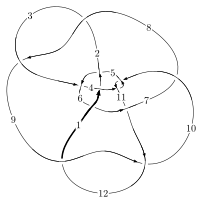
\includegraphics[width=112pt]{../../../GIT/diagram.site/Diagrams/png/1923_12a_1122.png}\\
\ \ \ A knot diagram\footnotemark}&
\allowdisplaybreaks
\textbf{Linearized knot diagam} \\
\cline{2-2}
 &
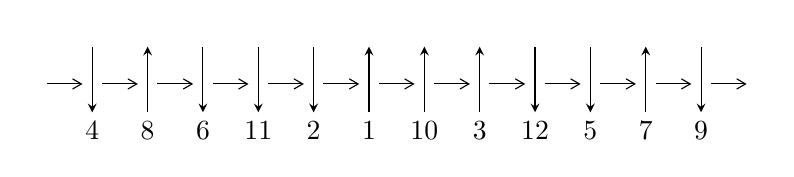
\begin{tikzpicture}[x=20pt, y=17pt]
	% nodes
	\node (C0) at (0, 0) {};
	\node (C1) at (1, 0) {};
	\node (C1U) at (1, +1) {};
	\node (C1D) at (1, -1) {4};

	\node (C2) at (2, 0) {};
	\node (C2U) at (2, +1) {};
	\node (C2D) at (2, -1) {8};

	\node (C3) at (3, 0) {};
	\node (C3U) at (3, +1) {};
	\node (C3D) at (3, -1) {6};

	\node (C4) at (4, 0) {};
	\node (C4U) at (4, +1) {};
	\node (C4D) at (4, -1) {11};

	\node (C5) at (5, 0) {};
	\node (C5U) at (5, +1) {};
	\node (C5D) at (5, -1) {2};

	\node (C6) at (6, 0) {};
	\node (C6U) at (6, +1) {};
	\node (C6D) at (6, -1) {1};

	\node (C7) at (7, 0) {};
	\node (C7U) at (7, +1) {};
	\node (C7D) at (7, -1) {10};

	\node (C8) at (8, 0) {};
	\node (C8U) at (8, +1) {};
	\node (C8D) at (8, -1) {3};

	\node (C9) at (9, 0) {};
	\node (C9U) at (9, +1) {};
	\node (C9D) at (9, -1) {12};

	\node (C10) at (10, 0) {};
	\node (C10U) at (10, +1) {};
	\node (C10D) at (10, -1) {5};

	\node (C11) at (11, 0) {};
	\node (C11U) at (11, +1) {};
	\node (C11D) at (11, -1) {7};

	\node (C12) at (12, 0) {};
	\node (C12U) at (12, +1) {};
	\node (C12D) at (12, -1) {9};
	\node (C13) at (13, 0) {};

	% arrows
	\draw[->,>={angle 60}]
	(C0) edge (C1) (C1) edge (C2) (C2) edge (C3) (C3) edge (C4) (C4) edge (C5) (C5) edge (C6) (C6) edge (C7) (C7) edge (C8) (C8) edge (C9) (C9) edge (C10) (C10) edge (C11) (C11) edge (C12) (C12) edge (C13) ;	\draw[->,>=stealth]
	(C1U) edge (C1D) (C2D) edge (C2U) (C3U) edge (C3D) (C4U) edge (C4D) (C5U) edge (C5D) (C6D) edge (C6U) (C7D) edge (C7U) (C8D) edge (C8U) (C9U) edge (C9D) (C10U) edge (C10D) (C11D) edge (C11U) (C12U) edge (C12D) ;
	\end{tikzpicture} \\
\hhline{~~} \\& 
\textbf{Solving Sequence} \\ \cline{2-2} 
 &
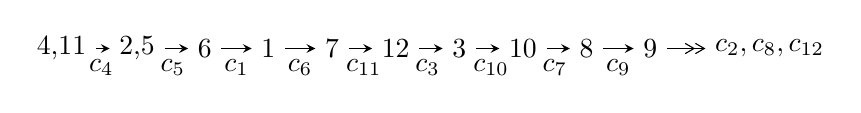
\begin{tikzpicture}[x=23pt, y=7pt]
	% node
	\node (A0) at (-1/8, 0) {4,11};
	\node (A1) at (17/16, 0) {2,5};
	\node (A2) at (17/8, 0) {6};
	\node (A3) at (25/8, 0) {1};
	\node (A4) at (33/8, 0) {7};
	\node (A5) at (41/8, 0) {12};
	\node (A6) at (49/8, 0) {3};
	\node (A7) at (57/8, 0) {10};
	\node (A8) at (65/8, 0) {8};
	\node (A9) at (73/8, 0) {9};
	\node (C1) at (1/2, -1) {$c_{4}$};
	\node (C2) at (13/8, -1) {$c_{5}$};
	\node (C3) at (21/8, -1) {$c_{1}$};
	\node (C4) at (29/8, -1) {$c_{6}$};
	\node (C5) at (37/8, -1) {$c_{11}$};
	\node (C6) at (45/8, -1) {$c_{3}$};
	\node (C7) at (53/8, -1) {$c_{10}$};
	\node (C8) at (61/8, -1) {$c_{7}$};
	\node (C9) at (69/8, -1) {$c_{9}$};
	\node (A10) at (11, 0) {$c_{2},c_{8},c_{12}$};

	% edge
	\draw[->,>=stealth]	
	(A0) edge (A1) (A1) edge (A2) (A2) edge (A3) (A3) edge (A4) (A4) edge (A5) (A5) edge (A6) (A6) edge (A7) (A7) edge (A8) (A8) edge (A9) ;
	\draw[->>,>={angle 60}]	
	(A9) edge (A10);
\end{tikzpicture} \\ 

\end{tabular} \\

\footnotetext{
The image of knot diagram is generated by the software ``\textbf{Draw programme}" developed by Andrew Bartholomew(\url{http://www.layer8.co.uk/maths/draw/index.htm\#Running-draw}), where we modified some parts for our purpose(\url{https://github.com/CATsTAILs/LinksPainter}).
}\phantom \\ \newline 
\centering \textbf{Ideals for irreducible components\footnotemark of $X_{\text{par}}$} 
 
\begin{align*}
I^u_{1}&=\langle 
6.83028\times10^{1161} u^{193}+3.53445\times10^{1162} u^{192}+\cdots+2.95981\times10^{1162} b-2.15705\times10^{1165},\\
\phantom{I^u_{1}}&\phantom{= \langle  }-4.50554\times10^{1164} u^{193}-1.12219\times10^{1165} u^{192}+\cdots+1.42367\times10^{1165} a+5.78965\times10^{1166},\\
\phantom{I^u_{1}}&\phantom{= \langle  }u^{194}+2 u^{193}+\cdots-655 u-481\rangle \\
I^u_{2}&=\langle 
-3.12959\times10^{52} u^{51}-1.42487\times10^{53} u^{50}+\cdots+2.34999\times10^{51} b+1.26295\times10^{53},\\
\phantom{I^u_{2}}&\phantom{= \langle  }-2.98795\times10^{53} u^{51}-7.64871\times10^{53} u^{50}+\cdots+2.34999\times10^{51} a-3.67199\times10^{53},\;u^{52}+3 u^{51}+\cdots+2 u-1\rangle \\
\\
\end{align*}
\raggedright * 2 irreducible components of $\dim_{\mathbb{C}}=0$, with total 246 representations.\\
\footnotetext{All coefficients of polynomials are rational numbers. But the coefficients are sometimes approximated in decimal forms when there is not enough margin.}
\newpage
\renewcommand{\arraystretch}{1}
\centering \section*{I. $I^u_{1}= \langle 6.83\times10^{1161} u^{193}+3.53\times10^{1162} u^{192}+\cdots+2.96\times10^{1162} b-2.16\times10^{1165},\;-4.51\times10^{1164} u^{193}-1.12\times10^{1165} u^{192}+\cdots+1.42\times10^{1165} a+5.79\times10^{1166},\;u^{194}+2 u^{193}+\cdots-655 u-481 \rangle$}
\flushleft \textbf{(i) Arc colorings}\\
\begin{tabular}{m{7pt} m{180pt} m{7pt} m{180pt} }
\flushright $a_{4}=$&$\begin{pmatrix}1\\0\end{pmatrix}$ \\
\flushright $a_{11}=$&$\begin{pmatrix}0\\u\end{pmatrix}$ \\
\flushright $a_{2}=$&$\begin{pmatrix}0.316474 u^{193}+0.788240 u^{192}+\cdots-9.52894 u-40.6671\\-0.230768 u^{193}-1.19415 u^{192}+\cdots+568.908 u+728.780\end{pmatrix}$ \\
\flushright $a_{5}=$&$\begin{pmatrix}1\\u^2\end{pmatrix}$ \\
\flushright $a_{6}=$&$\begin{pmatrix}-0.162671 u^{193}+0.448121 u^{192}+\cdots-776.891 u-100.653\\0.475182 u^{193}+0.876579 u^{192}+\cdots-738.805 u-41.3730\end{pmatrix}$ \\
\flushright $a_{1}=$&$\begin{pmatrix}0.0857068 u^{193}-0.405910 u^{192}+\cdots+559.379 u+688.113\\-0.230768 u^{193}-1.19415 u^{192}+\cdots+568.908 u+728.780\end{pmatrix}$ \\
\flushright $a_{7}=$&$\begin{pmatrix}-0.150675 u^{193}+0.396798 u^{192}+\cdots+135.660 u-612.208\\-0.591702 u^{193}-1.82715 u^{192}+\cdots+908.617 u+439.357\end{pmatrix}$ \\
\flushright $a_{12}=$&$\begin{pmatrix}-0.474308 u^{193}-0.715475 u^{192}+\cdots-98.9571 u-404.517\\0.0961734 u^{193}+0.932923 u^{192}+\cdots-498.590 u-649.306\end{pmatrix}$ \\
\flushright $a_{3}=$&$\begin{pmatrix}-0.112320 u^{193}-1.26756 u^{192}+\cdots+686.156 u+1013.43\\-0.100660 u^{193}-0.241166 u^{192}+\cdots+182.458 u+206.095\end{pmatrix}$ \\
\flushright $a_{10}=$&$\begin{pmatrix}u\\u^3+u\end{pmatrix}$ \\
\flushright $a_{8}=$&$\begin{pmatrix}0.321414 u^{193}+1.89657 u^{192}+\cdots-640.002 u-1102.47\\-0.533946 u^{193}-1.41798 u^{192}+\cdots+723.942 u+216.338\end{pmatrix}$ \\
\flushright $a_{9}=$&$\begin{pmatrix}0.459020 u^{193}+1.16878 u^{192}+\cdots-543.442 u-65.5094\\-1.08933 u^{193}-2.21471 u^{192}+\cdots+1271.97 u+134.816\end{pmatrix}$\\&\end{tabular}
\flushleft \textbf{(ii) Obstruction class $= -1$}\\~\\
\flushleft \textbf{(iii) Cusp Shapes $= 4.49255 u^{193}+7.09007 u^{192}+\cdots-1628.95 u+1786.25$}\\~\\
\newpage\renewcommand{\arraystretch}{1}
\flushleft \textbf{(iv) u-Polynomials at the component}\newline \\
\begin{tabular}{m{50pt}|m{274pt}}
Crossings & \hspace{64pt}u-Polynomials at each crossing \\
\hline $$\begin{aligned}c_{1}\end{aligned}$$&$\begin{aligned}
&u^{194}-22 u^{193}+\cdots-21 u-2
\end{aligned}$\\
\hline $$\begin{aligned}c_{2},c_{8}\end{aligned}$$&$\begin{aligned}
&u^{194}+7 u^{193}+\cdots+54430 u+211369
\end{aligned}$\\
\hline $$\begin{aligned}c_{3}\end{aligned}$$&$\begin{aligned}
&u^{194}-23 u^{193}+\cdots-122 u+4
\end{aligned}$\\
\hline $$\begin{aligned}c_{4},c_{10}\end{aligned}$$&$\begin{aligned}
&u^{194}-2 u^{193}+\cdots+655 u-481
\end{aligned}$\\
\hline $$\begin{aligned}c_{5}\end{aligned}$$&$\begin{aligned}
&u^{194}+2 u^{193}+\cdots+401163 u-24353
\end{aligned}$\\
\hline $$\begin{aligned}c_{6}\end{aligned}$$&$\begin{aligned}
&u^{194}+4 u^{193}+\cdots-5730703 u-207001
\end{aligned}$\\
\hline $$\begin{aligned}c_{7}\end{aligned}$$&$\begin{aligned}
&u^{194}+3 u^{193}+\cdots+15352307260 u+814469648
\end{aligned}$\\
\hline $$\begin{aligned}c_{9},c_{12}\end{aligned}$$&$\begin{aligned}
&u^{194}-7 u^{193}+\cdots-2210969 u+115748
\end{aligned}$\\
\hline $$\begin{aligned}c_{11}\end{aligned}$$&$\begin{aligned}
&u^{194}-16 u^{193}+\cdots-988503 u+59801
\end{aligned}$\\
\hline
\end{tabular}\\~\\
\newpage\renewcommand{\arraystretch}{1}
\flushleft \textbf{(v) Riley Polynomials at the component}\newline \\
\begin{tabular}{m{50pt}|m{274pt}}
Crossings & \hspace{64pt}Riley Polynomials at each crossing \\
\hline $$\begin{aligned}c_{1}\end{aligned}$$&$\begin{aligned}
&y^{194}-12 y^{193}+\cdots+111 y+4
\end{aligned}$\\
\hline $$\begin{aligned}c_{2},c_{8}\end{aligned}$$&$\begin{aligned}
&y^{194}-131 y^{193}+\cdots-1961771990150 y+44676854161
\end{aligned}$\\
\hline $$\begin{aligned}c_{3}\end{aligned}$$&$\begin{aligned}
&y^{194}-55 y^{193}+\cdots-2140 y+16
\end{aligned}$\\
\hline $$\begin{aligned}c_{4},c_{10}\end{aligned}$$&$\begin{aligned}
&y^{194}+110 y^{193}+\cdots+12580101 y+231361
\end{aligned}$\\
\hline $$\begin{aligned}c_{5}\end{aligned}$$&$\begin{aligned}
&y^{194}-34 y^{193}+\cdots+42235244289 y+593068609
\end{aligned}$\\
\hline $$\begin{aligned}c_{6}\end{aligned}$$&$\begin{aligned}
&y^{194}+26 y^{193}+\cdots-729590165583 y+42849414001
\end{aligned}$\\
\hline $$\begin{aligned}c_{7}\end{aligned}$$&$\begin{aligned}
&y^{194}-17 y^{193}+\cdots-1.29\times10^{20} y+6.63\times10^{17}
\end{aligned}$\\
\hline $$\begin{aligned}c_{9},c_{12}\end{aligned}$$&$\begin{aligned}
&y^{194}+117 y^{193}+\cdots-316216846553 y+13397599504
\end{aligned}$\\
\hline $$\begin{aligned}c_{11}\end{aligned}$$&$\begin{aligned}
&y^{194}+52 y^{193}+\cdots-607267799989 y+3576159601
\end{aligned}$\\
\hline
\end{tabular}\\~\\
\newpage\flushleft \textbf{(vi) Complex Volumes and Cusp Shapes}
$$\begin{array}{c|c|c}  
\text{Solutions to }I^u_{1}& \I (\text{vol} + \sqrt{-1}CS) & \text{Cusp shape}\\
 \hline 
\begin{aligned}
u &= -0.251757 + 1.005160 I \\
a &= \phantom{-}0.065670 - 0.814168 I \\
b &= \phantom{-}0.784624 + 0.726243 I\end{aligned}
 & \phantom{-}4.03911 - 1.81200 I & \phantom{-0.000000 } 0 \\ \hline\begin{aligned}
u &= -0.251757 - 1.005160 I \\
a &= \phantom{-}0.065670 + 0.814168 I \\
b &= \phantom{-}0.784624 - 0.726243 I\end{aligned}
 & \phantom{-}4.03911 + 1.81200 I & \phantom{-0.000000 } 0 \\ \hline\begin{aligned}
u &= \phantom{-}0.982645 + 0.329574 I \\
a &= -0.089178 + 0.212648 I \\
b &= -1.04301 + 0.95954 I\end{aligned}
 & -0.06974 + 8.80865 I & \phantom{-0.000000 } 0 \\ \hline\begin{aligned}
u &= \phantom{-}0.982645 - 0.329574 I \\
a &= -0.089178 - 0.212648 I \\
b &= -1.04301 - 0.95954 I\end{aligned}
 & -0.06974 - 8.80865 I & \phantom{-0.000000 } 0 \\ \hline\begin{aligned}
u &= \phantom{-}0.214125 + 0.931248 I \\
a &= \phantom{-}0.17891 + 2.39952 I \\
b &= -1.214160 - 0.313275 I\end{aligned}
 & \phantom{-}1.36282 - 0.88962 I & \phantom{-0.000000 } 0 \\ \hline\begin{aligned}
u &= \phantom{-}0.214125 - 0.931248 I \\
a &= \phantom{-}0.17891 - 2.39952 I \\
b &= -1.214160 + 0.313275 I\end{aligned}
 & \phantom{-}1.36282 + 0.88962 I & \phantom{-0.000000 } 0 \\ \hline\begin{aligned}
u &= \phantom{-}1.016210 + 0.324273 I \\
a &= \phantom{-}0.627073 + 0.384093 I \\
b &= \phantom{-}0.032360 + 0.930651 I\end{aligned}
 & -1.06555 - 1.00391 I & \phantom{-0.000000 } 0 \\ \hline\begin{aligned}
u &= \phantom{-}1.016210 - 0.324273 I \\
a &= \phantom{-}0.627073 - 0.384093 I \\
b &= \phantom{-}0.032360 - 0.930651 I\end{aligned}
 & -1.06555 + 1.00391 I & \phantom{-0.000000 } 0 \\ \hline\begin{aligned}
u &= -0.466839 + 0.962731 I \\
a &= \phantom{-}0.010936 + 0.805791 I \\
b &= \phantom{-}0.626339 - 0.682521 I\end{aligned}
 & \phantom{-}1.85805 - 0.72164 I & \phantom{-0.000000 } 0 \\ \hline\begin{aligned}
u &= -0.466839 - 0.962731 I \\
a &= \phantom{-}0.010936 - 0.805791 I \\
b &= \phantom{-}0.626339 + 0.682521 I\end{aligned}
 & \phantom{-}1.85805 + 0.72164 I & \phantom{-0.000000 } 0\\
 \hline 
 \end{array}$$\newpage$$\begin{array}{c|c|c}  
\text{Solutions to }I^u_{1}& \I (\text{vol} + \sqrt{-1}CS) & \text{Cusp shape}\\
 \hline 
\begin{aligned}
u &= \phantom{-}0.142704 + 1.060990 I \\
a &= \phantom{-}1.249840 - 0.221762 I \\
b &= -0.141575 + 0.260256 I\end{aligned}
 & \phantom{-}3.36336 + 0.09849 I & \phantom{-0.000000 } 0 \\ \hline\begin{aligned}
u &= \phantom{-}0.142704 - 1.060990 I \\
a &= \phantom{-}1.249840 + 0.221762 I \\
b &= -0.141575 - 0.260256 I\end{aligned}
 & \phantom{-}3.36336 - 0.09849 I & \phantom{-0.000000 } 0 \\ \hline\begin{aligned}
u &= -1.011830 + 0.360670 I \\
a &= -0.367858 + 0.687191 I \\
b &= -0.076766 + 0.307025 I\end{aligned}
 & -0.62929 + 4.73327 I & \phantom{-0.000000 } 0 \\ \hline\begin{aligned}
u &= -1.011830 - 0.360670 I \\
a &= -0.367858 - 0.687191 I \\
b &= -0.076766 - 0.307025 I\end{aligned}
 & -0.62929 - 4.73327 I & \phantom{-0.000000 } 0 \\ \hline\begin{aligned}
u &= \phantom{-}0.695188 + 0.607820 I \\
a &= \phantom{-}0.804761 - 0.198197 I \\
b &= \phantom{-}0.416918 + 0.116699 I\end{aligned}
 & -1.45350 - 1.59800 I & \phantom{-0.000000 } 0 \\ \hline\begin{aligned}
u &= \phantom{-}0.695188 - 0.607820 I \\
a &= \phantom{-}0.804761 + 0.198197 I \\
b &= \phantom{-}0.416918 - 0.116699 I\end{aligned}
 & -1.45350 + 1.59800 I & \phantom{-0.000000 } 0 \\ \hline\begin{aligned}
u &= -0.205871 + 1.064520 I \\
a &= \phantom{-}0.571788 + 1.131920 I \\
b &= \phantom{-}0.003233 - 1.157660 I\end{aligned}
 & \phantom{-}1.92174 - 1.25353 I & \phantom{-0.000000 } 0 \\ \hline\begin{aligned}
u &= -0.205871 - 1.064520 I \\
a &= \phantom{-}0.571788 - 1.131920 I \\
b &= \phantom{-}0.003233 + 1.157660 I\end{aligned}
 & \phantom{-}1.92174 + 1.25353 I & \phantom{-0.000000 } 0 \\ \hline\begin{aligned}
u &= -1.000960 + 0.429068 I \\
a &= \phantom{-}0.098914 - 0.204224 I \\
b &= -0.993434 - 0.939438 I\end{aligned}
 & -3.87014 - 3.52468 I & \phantom{-0.000000 } 0 \\ \hline\begin{aligned}
u &= -1.000960 - 0.429068 I \\
a &= \phantom{-}0.098914 + 0.204224 I \\
b &= -0.993434 + 0.939438 I\end{aligned}
 & -3.87014 + 3.52468 I & \phantom{-0.000000 } 0\\
 \hline 
 \end{array}$$\newpage$$\begin{array}{c|c|c}  
\text{Solutions to }I^u_{1}& \I (\text{vol} + \sqrt{-1}CS) & \text{Cusp shape}\\
 \hline 
\begin{aligned}
u &= \phantom{-}0.581094 + 0.682495 I \\
a &= -0.03382 + 1.58535 I \\
b &= -1.41985 + 0.32895 I\end{aligned}
 & -0.14014 - 2.35529 I & \phantom{-0.000000 } 0 \\ \hline\begin{aligned}
u &= \phantom{-}0.581094 - 0.682495 I \\
a &= -0.03382 - 1.58535 I \\
b &= -1.41985 - 0.32895 I\end{aligned}
 & -0.14014 + 2.35529 I & \phantom{-0.000000 } 0 \\ \hline\begin{aligned}
u &= -0.035267 + 0.886965 I \\
a &= -3.33799 - 1.21350 I \\
b &= -1.060060 + 0.000013 I\end{aligned}
 & \phantom{-}1.318930 + 0.093399 I & \phantom{-0.000000 } 0 \\ \hline\begin{aligned}
u &= -0.035267 - 0.886965 I \\
a &= -3.33799 + 1.21350 I \\
b &= -1.060060 - 0.000013 I\end{aligned}
 & \phantom{-}1.318930 - 0.093399 I & \phantom{-0.000000 } 0 \\ \hline\begin{aligned}
u &= \phantom{-}0.675575 + 0.563993 I \\
a &= \phantom{-}0.480160 - 0.101867 I \\
b &= \phantom{-}0.858190 + 0.463965 I\end{aligned}
 & -1.07794 - 4.33467 I & \phantom{-0.000000 } 0 \\ \hline\begin{aligned}
u &= \phantom{-}0.675575 - 0.563993 I \\
a &= \phantom{-}0.480160 + 0.101867 I \\
b &= \phantom{-}0.858190 - 0.463965 I\end{aligned}
 & -1.07794 + 4.33467 I & \phantom{-0.000000 } 0 \\ \hline\begin{aligned}
u &= -0.437100 + 0.757607 I \\
a &= \phantom{-}0.394151 - 1.144180 I \\
b &= -1.395330 + 0.216322 I\end{aligned}
 & -1.70778 + 1.90491 I & \phantom{-0.000000 } 0 \\ \hline\begin{aligned}
u &= -0.437100 - 0.757607 I \\
a &= \phantom{-}0.394151 + 1.144180 I \\
b &= -1.395330 - 0.216322 I\end{aligned}
 & -1.70778 - 1.90491 I & \phantom{-0.000000 } 0 \\ \hline\begin{aligned}
u &= -0.358107 + 0.793890 I \\
a &= -0.23246 - 2.99667 I \\
b &= -1.07614 + 1.32262 I\end{aligned}
 & -2.91397 + 3.60701 I & \phantom{-0.000000 } 0 \\ \hline\begin{aligned}
u &= -0.358107 - 0.793890 I \\
a &= -0.23246 + 2.99667 I \\
b &= -1.07614 - 1.32262 I\end{aligned}
 & -2.91397 - 3.60701 I & \phantom{-0.000000 } 0\\
 \hline 
 \end{array}$$\newpage$$\begin{array}{c|c|c}  
\text{Solutions to }I^u_{1}& \I (\text{vol} + \sqrt{-1}CS) & \text{Cusp shape}\\
 \hline 
\begin{aligned}
u &= -0.813563 + 0.301681 I \\
a &= \phantom{-}0.901564 + 0.426122 I \\
b &= \phantom{-}0.922462 - 0.846918 I\end{aligned}
 & \phantom{-}6.20018 + 4.65473 I & \phantom{-0.000000 } 0 \\ \hline\begin{aligned}
u &= -0.813563 - 0.301681 I \\
a &= \phantom{-}0.901564 - 0.426122 I \\
b &= \phantom{-}0.922462 + 0.846918 I\end{aligned}
 & \phantom{-}6.20018 - 4.65473 I & \phantom{-0.000000 } 0 \\ \hline\begin{aligned}
u &= \phantom{-}0.460993 + 1.036090 I \\
a &= -1.02603 + 1.24171 I \\
b &= \phantom{-}0.172390 - 0.889229 I\end{aligned}
 & \phantom{-}6.88693 - 5.93163 I & \phantom{-0.000000 } 0 \\ \hline\begin{aligned}
u &= \phantom{-}0.460993 - 1.036090 I \\
a &= -1.02603 - 1.24171 I \\
b &= \phantom{-}0.172390 + 0.889229 I\end{aligned}
 & \phantom{-}6.88693 + 5.93163 I & \phantom{-0.000000 } 0 \\ \hline\begin{aligned}
u &= -0.391002 + 0.769934 I \\
a &= \phantom{-}0.735209 - 0.288979 I \\
b &= -1.47650 - 0.63202 I\end{aligned}
 & -2.93391 - 0.21259 I & \phantom{-0.000000 } 0 \\ \hline\begin{aligned}
u &= -0.391002 - 0.769934 I \\
a &= \phantom{-}0.735209 + 0.288979 I \\
b &= -1.47650 + 0.63202 I\end{aligned}
 & -2.93391 + 0.21259 I & \phantom{-0.000000 } 0 \\ \hline\begin{aligned}
u &= -0.926219 + 0.668024 I \\
a &= \phantom{-}0.275549 - 0.081834 I \\
b &= \phantom{-}1.025130 + 0.828927 I\end{aligned}
 & \phantom{-}5.94711 - 1.70630 I & \phantom{-0.000000 } 0 \\ \hline\begin{aligned}
u &= -0.926219 - 0.668024 I \\
a &= \phantom{-}0.275549 + 0.081834 I \\
b &= \phantom{-}1.025130 - 0.828927 I\end{aligned}
 & \phantom{-}5.94711 + 1.70630 I & \phantom{-0.000000 } 0 \\ \hline\begin{aligned}
u &= \phantom{-}0.348413 + 1.088770 I \\
a &= \phantom{-}0.21746 + 1.82743 I \\
b &= -0.445118 - 0.732955 I\end{aligned}
 & \phantom{-}1.70078 - 3.28764 I & \phantom{-0.000000 } 0 \\ \hline\begin{aligned}
u &= \phantom{-}0.348413 - 1.088770 I \\
a &= \phantom{-}0.21746 - 1.82743 I \\
b &= -0.445118 + 0.732955 I\end{aligned}
 & \phantom{-}1.70078 + 3.28764 I & \phantom{-0.000000 } 0\\
 \hline 
 \end{array}$$\newpage$$\begin{array}{c|c|c}  
\text{Solutions to }I^u_{1}& \I (\text{vol} + \sqrt{-1}CS) & \text{Cusp shape}\\
 \hline 
\begin{aligned}
u &= \phantom{-}0.532150 + 1.013340 I \\
a &= \phantom{-}1.235190 - 0.307355 I \\
b &= \phantom{-}0.702682 + 0.002432 I\end{aligned}
 & -0.58052 - 2.49187 I & \phantom{-0.000000 } 0 \\ \hline\begin{aligned}
u &= \phantom{-}0.532150 - 1.013340 I \\
a &= \phantom{-}1.235190 + 0.307355 I \\
b &= \phantom{-}0.702682 - 0.002432 I\end{aligned}
 & -0.58052 + 2.49187 I & \phantom{-0.000000 } 0 \\ \hline\begin{aligned}
u &= \phantom{-}0.655997 + 0.539418 I \\
a &= -1.54703 + 2.38776 I \\
b &= -0.636474 - 0.980063 I\end{aligned}
 & \phantom{-}1.92121 - 7.90604 I & \phantom{-0.000000 } 0 \\ \hline\begin{aligned}
u &= \phantom{-}0.655997 - 0.539418 I \\
a &= -1.54703 - 2.38776 I \\
b &= -0.636474 + 0.980063 I\end{aligned}
 & \phantom{-}1.92121 + 7.90604 I & \phantom{-0.000000 } 0 \\ \hline\begin{aligned}
u &= -0.455534 + 1.059860 I \\
a &= \phantom{-}0.831829 + 0.882654 I \\
b &= \phantom{-}0.318891 - 0.567994 I\end{aligned}
 & \phantom{-}4.56429 + 1.17523 I & \phantom{-0.000000 } 0 \\ \hline\begin{aligned}
u &= -0.455534 - 1.059860 I \\
a &= \phantom{-}0.831829 - 0.882654 I \\
b &= \phantom{-}0.318891 + 0.567994 I\end{aligned}
 & \phantom{-}4.56429 - 1.17523 I & \phantom{-0.000000 } 0 \\ \hline\begin{aligned}
u &= \phantom{-}0.275915 + 1.128450 I \\
a &= \phantom{-}1.07197 - 1.90078 I \\
b &= -0.22836 + 2.54503 I\end{aligned}
 & \phantom{-}4.41088 - 3.93533 I & \phantom{-0.000000 } 0 \\ \hline\begin{aligned}
u &= \phantom{-}0.275915 - 1.128450 I \\
a &= \phantom{-}1.07197 + 1.90078 I \\
b &= -0.22836 - 2.54503 I\end{aligned}
 & \phantom{-}4.41088 + 3.93533 I & \phantom{-0.000000 } 0 \\ \hline\begin{aligned}
u &= \phantom{-}0.533836 + 1.032400 I \\
a &= -0.21871 + 2.01027 I \\
b &= -0.86923 - 1.23646 I\end{aligned}
 & \phantom{-}1.27643 - 6.55006 I & \phantom{-0.000000 } 0 \\ \hline\begin{aligned}
u &= \phantom{-}0.533836 - 1.032400 I \\
a &= -0.21871 - 2.01027 I \\
b &= -0.86923 + 1.23646 I\end{aligned}
 & \phantom{-}1.27643 + 6.55006 I & \phantom{-0.000000 } 0\\
 \hline 
 \end{array}$$\newpage$$\begin{array}{c|c|c}  
\text{Solutions to }I^u_{1}& \I (\text{vol} + \sqrt{-1}CS) & \text{Cusp shape}\\
 \hline 
\begin{aligned}
u &= \phantom{-}0.036235 + 0.828297 I \\
a &= -1.96273 + 3.19554 I \\
b &= \phantom{-}1.13058 - 1.96038 I\end{aligned}
 & \phantom{-}2.63815 + 2.68431 I & \phantom{-0.000000 } 0 \\ \hline\begin{aligned}
u &= \phantom{-}0.036235 - 0.828297 I \\
a &= -1.96273 - 3.19554 I \\
b &= \phantom{-}1.13058 + 1.96038 I\end{aligned}
 & \phantom{-}2.63815 - 2.68431 I & \phantom{-0.000000 } 0 \\ \hline\begin{aligned}
u &= -0.470313 + 0.682009 I \\
a &= \phantom{-}0.566573 - 0.297380 I \\
b &= \phantom{-}0.894658 - 0.369987 I\end{aligned}
 & \phantom{-}0.54606 + 8.15873 I & \phantom{-0.000000 } 0 \\ \hline\begin{aligned}
u &= -0.470313 - 0.682009 I \\
a &= \phantom{-}0.566573 + 0.297380 I \\
b &= \phantom{-}0.894658 + 0.369987 I\end{aligned}
 & \phantom{-}0.54606 - 8.15873 I & \phantom{-0.000000 } 0 \\ \hline\begin{aligned}
u &= -0.341596 + 1.143730 I \\
a &= \phantom{-}0.09640 - 1.62274 I \\
b &= -0.259770 + 1.095630 I\end{aligned}
 & \phantom{-}5.14834 + 6.58962 I & \phantom{-0.000000 } 0 \\ \hline\begin{aligned}
u &= -0.341596 - 1.143730 I \\
a &= \phantom{-}0.09640 + 1.62274 I \\
b &= -0.259770 - 1.095630 I\end{aligned}
 & \phantom{-}5.14834 - 6.58962 I & \phantom{-0.000000 } 0 \\ \hline\begin{aligned}
u &= -0.406600 + 1.126390 I \\
a &= -0.10381 + 2.06162 I \\
b &= \phantom{-}0.86777 - 1.26956 I\end{aligned}
 & \phantom{-}3.47689 + 10.61870 I & \phantom{-0.000000 } 0 \\ \hline\begin{aligned}
u &= -0.406600 - 1.126390 I \\
a &= -0.10381 - 2.06162 I \\
b &= \phantom{-}0.86777 + 1.26956 I\end{aligned}
 & \phantom{-}3.47689 - 10.61870 I & \phantom{-0.000000 } 0 \\ \hline\begin{aligned}
u &= -0.561963 + 1.059780 I \\
a &= -0.07886 - 1.86346 I \\
b &= -1.00344 + 1.26714 I\end{aligned}
 & \phantom{-}0.25235 + 6.31362 I & \phantom{-0.000000 } 0 \\ \hline\begin{aligned}
u &= -0.561963 - 1.059780 I \\
a &= -0.07886 + 1.86346 I \\
b &= -1.00344 - 1.26714 I\end{aligned}
 & \phantom{-}0.25235 - 6.31362 I & \phantom{-0.000000 } 0\\
 \hline 
 \end{array}$$\newpage$$\begin{array}{c|c|c}  
\text{Solutions to }I^u_{1}& \I (\text{vol} + \sqrt{-1}CS) & \text{Cusp shape}\\
 \hline 
\begin{aligned}
u &= -0.660346 + 0.442981 I \\
a &= \phantom{-}0.752524 - 0.156516 I \\
b &= -1.155490 - 0.678625 I\end{aligned}
 & -1.53901 - 1.54155 I & \phantom{-0.000000 } 0 \\ \hline\begin{aligned}
u &= -0.660346 - 0.442981 I \\
a &= \phantom{-}0.752524 + 0.156516 I \\
b &= -1.155490 + 0.678625 I\end{aligned}
 & -1.53901 + 1.54155 I & \phantom{-0.000000 } 0 \\ \hline\begin{aligned}
u &= \phantom{-}0.402563 + 1.136740 I \\
a &= -1.54278 + 0.22746 I \\
b &= -0.730058 - 0.174551 I\end{aligned}
 & \phantom{-}5.39371 - 10.74820 I & \phantom{-0.000000 } 0 \\ \hline\begin{aligned}
u &= \phantom{-}0.402563 - 1.136740 I \\
a &= -1.54278 - 0.22746 I \\
b &= -0.730058 + 0.174551 I\end{aligned}
 & \phantom{-}5.39371 + 10.74820 I & \phantom{-0.000000 } 0 \\ \hline\begin{aligned}
u &= \phantom{-}0.479135 + 1.109900 I \\
a &= -1.28307 + 0.66570 I \\
b &= -0.177953 - 0.323546 I\end{aligned}
 & \phantom{-}8.29510 + 2.72233 I & \phantom{-0.000000 } 0 \\ \hline\begin{aligned}
u &= \phantom{-}0.479135 - 1.109900 I \\
a &= -1.28307 - 0.66570 I \\
b &= -0.177953 + 0.323546 I\end{aligned}
 & \phantom{-}8.29510 - 2.72233 I & \phantom{-0.000000 } 0 \\ \hline\begin{aligned}
u &= \phantom{-}0.422627 + 1.136010 I \\
a &= \phantom{-}0.68700 - 1.80083 I \\
b &= \phantom{-}0.514403 + 1.028580 I\end{aligned}
 & \phantom{-}7.17178 - 1.49381 I & \phantom{-0.000000 } 0 \\ \hline\begin{aligned}
u &= \phantom{-}0.422627 - 1.136010 I \\
a &= \phantom{-}0.68700 + 1.80083 I \\
b &= \phantom{-}0.514403 - 1.028580 I\end{aligned}
 & \phantom{-}7.17178 + 1.49381 I & \phantom{-0.000000 } 0 \\ \hline\begin{aligned}
u &= -0.101135 + 0.777690 I \\
a &= -0.67397 + 2.30455 I \\
b &= -0.638774 - 0.859690 I\end{aligned}
 & \phantom{-}3.29137 - 4.87853 I & \phantom{-0.000000 } 0 \\ \hline\begin{aligned}
u &= -0.101135 - 0.777690 I \\
a &= -0.67397 - 2.30455 I \\
b &= -0.638774 + 0.859690 I\end{aligned}
 & \phantom{-}3.29137 + 4.87853 I & \phantom{-0.000000 } 0\\
 \hline 
 \end{array}$$\newpage$$\begin{array}{c|c|c}  
\text{Solutions to }I^u_{1}& \I (\text{vol} + \sqrt{-1}CS) & \text{Cusp shape}\\
 \hline 
\begin{aligned}
u &= \phantom{-}0.483201 + 1.115950 I \\
a &= \phantom{-}0.17849 - 2.05038 I \\
b &= \phantom{-}0.238144 + 0.980695 I\end{aligned}
 & \phantom{-}8.15546 - 10.17690 I & \phantom{-0.000000 } 0 \\ \hline\begin{aligned}
u &= \phantom{-}0.483201 - 1.115950 I \\
a &= \phantom{-}0.17849 + 2.05038 I \\
b &= \phantom{-}0.238144 - 0.980695 I\end{aligned}
 & \phantom{-}8.15546 + 10.17690 I & \phantom{-0.000000 } 0 \\ \hline\begin{aligned}
u &= \phantom{-}0.383884 + 1.160880 I \\
a &= -0.18599 - 1.91854 I \\
b &= \phantom{-}1.12618 + 1.17427 I\end{aligned}
 & \phantom{-}2.83127 - 7.17967 I & \phantom{-0.000000 } 0 \\ \hline\begin{aligned}
u &= \phantom{-}0.383884 - 1.160880 I \\
a &= -0.18599 + 1.91854 I \\
b &= \phantom{-}1.12618 - 1.17427 I\end{aligned}
 & \phantom{-}2.83127 + 7.17967 I & \phantom{-0.000000 } 0 \\ \hline\begin{aligned}
u &= \phantom{-}0.172112 + 1.211690 I \\
a &= \phantom{-}0.755991 - 1.051400 I \\
b &= -0.449115 + 1.251620 I\end{aligned}
 & \phantom{-}5.69232 + 5.44735 I & \phantom{-0.000000 } 0 \\ \hline\begin{aligned}
u &= \phantom{-}0.172112 - 1.211690 I \\
a &= \phantom{-}0.755991 + 1.051400 I \\
b &= -0.449115 - 1.251620 I\end{aligned}
 & \phantom{-}5.69232 - 5.44735 I & \phantom{-0.000000 } 0 \\ \hline\begin{aligned}
u &= -0.570904 + 0.515951 I \\
a &= \phantom{-}0.792513 + 1.150750 I \\
b &= \phantom{-}0.238179 + 0.297075 I\end{aligned}
 & \phantom{-}0.25463 - 3.43709 I & \phantom{-0.000000 } 0 \\ \hline\begin{aligned}
u &= -0.570904 - 0.515951 I \\
a &= \phantom{-}0.792513 - 1.150750 I \\
b &= \phantom{-}0.238179 - 0.297075 I\end{aligned}
 & \phantom{-}0.25463 + 3.43709 I & \phantom{-0.000000 } 0 \\ \hline\begin{aligned}
u &= \phantom{-}0.249545 + 0.726358 I \\
a &= \phantom{-}0.79812 + 1.71675 I \\
b &= -0.710597 - 0.173236 I\end{aligned}
 & -0.16323 - 2.68133 I & \phantom{-0.000000 } 0 \\ \hline\begin{aligned}
u &= \phantom{-}0.249545 - 0.726358 I \\
a &= \phantom{-}0.79812 - 1.71675 I \\
b &= -0.710597 + 0.173236 I\end{aligned}
 & -0.16323 + 2.68133 I & \phantom{-0.000000 } 0\\
 \hline 
 \end{array}$$\newpage$$\begin{array}{c|c|c}  
\text{Solutions to }I^u_{1}& \I (\text{vol} + \sqrt{-1}CS) & \text{Cusp shape}\\
 \hline 
\begin{aligned}
u &= -0.348831 + 1.186080 I \\
a &= \phantom{-}0.30683 + 1.61592 I \\
b &= \phantom{-}0.557400 - 0.988723 I\end{aligned}
 & \phantom{-}5.76630 + 2.12507 I & \phantom{-0.000000 } 0 \\ \hline\begin{aligned}
u &= -0.348831 - 1.186080 I \\
a &= \phantom{-}0.30683 - 1.61592 I \\
b &= \phantom{-}0.557400 + 0.988723 I\end{aligned}
 & \phantom{-}5.76630 - 2.12507 I & \phantom{-0.000000 } 0 \\ \hline\begin{aligned}
u &= -0.097341 + 0.757181 I \\
a &= -2.06523 - 1.15859 I \\
b &= \phantom{-}1.54580 + 0.48323 I\end{aligned}
 & \phantom{-}0.78761 + 3.26692 I & \phantom{-0.000000 } 0 \\ \hline\begin{aligned}
u &= -0.097341 - 0.757181 I \\
a &= -2.06523 + 1.15859 I \\
b &= \phantom{-}1.54580 - 0.48323 I\end{aligned}
 & \phantom{-}0.78761 - 3.26692 I & \phantom{-0.000000 } 0 \\ \hline\begin{aligned}
u &= -0.203585 + 1.222570 I \\
a &= \phantom{-}0.867811 - 0.804950 I \\
b &= -0.405179 + 0.098559 I\end{aligned}
 & \phantom{-}3.04210 + 0.35319 I & \phantom{-0.000000 } 0 \\ \hline\begin{aligned}
u &= -0.203585 - 1.222570 I \\
a &= \phantom{-}0.867811 + 0.804950 I \\
b &= -0.405179 - 0.098559 I\end{aligned}
 & \phantom{-}3.04210 - 0.35319 I & \phantom{-0.000000 } 0 \\ \hline\begin{aligned}
u &= \phantom{-}0.634954 + 1.069320 I \\
a &= \phantom{-}0.488721 - 0.743619 I \\
b &= \phantom{-}0.505751 + 0.360321 I\end{aligned}
 & -0.15354 - 3.57414 I & \phantom{-0.000000 } 0 \\ \hline\begin{aligned}
u &= \phantom{-}0.634954 - 1.069320 I \\
a &= \phantom{-}0.488721 + 0.743619 I \\
b &= \phantom{-}0.505751 - 0.360321 I\end{aligned}
 & -0.15354 + 3.57414 I & \phantom{-0.000000 } 0 \\ \hline\begin{aligned}
u &= -1.206010 + 0.331830 I \\
a &= \phantom{-}0.0558816 - 0.0711270 I \\
b &= \phantom{-}0.990725 + 0.978209 I\end{aligned}
 & \phantom{-}3.0478 - 14.9833 I & \phantom{-0.000000 } 0 \\ \hline\begin{aligned}
u &= -1.206010 - 0.331830 I \\
a &= \phantom{-}0.0558816 + 0.0711270 I \\
b &= \phantom{-}0.990725 - 0.978209 I\end{aligned}
 & \phantom{-}3.0478 + 14.9833 I & \phantom{-0.000000 } 0\\
 \hline 
 \end{array}$$\newpage$$\begin{array}{c|c|c}  
\text{Solutions to }I^u_{1}& \I (\text{vol} + \sqrt{-1}CS) & \text{Cusp shape}\\
 \hline 
\begin{aligned}
u &= \phantom{-}0.058524 + 0.744824 I \\
a &= -1.43585 - 0.89582 I \\
b &= -0.869890 + 0.351887 I\end{aligned}
 & -0.301261 + 1.229510 I & \phantom{-0.000000 } 0 \\ \hline\begin{aligned}
u &= \phantom{-}0.058524 - 0.744824 I \\
a &= -1.43585 + 0.89582 I \\
b &= -0.869890 - 0.351887 I\end{aligned}
 & -0.301261 - 1.229510 I & \phantom{-0.000000 } 0 \\ \hline\begin{aligned}
u &= -0.601500 + 1.099960 I \\
a &= \phantom{-}0.681507 + 0.857407 I \\
b &= \phantom{-}0.654376 - 0.371350 I\end{aligned}
 & \phantom{-}1.76952 + 8.45386 I & \phantom{-0.000000 } 0 \\ \hline\begin{aligned}
u &= -0.601500 - 1.099960 I \\
a &= \phantom{-}0.681507 - 0.857407 I \\
b &= \phantom{-}0.654376 + 0.371350 I\end{aligned}
 & \phantom{-}1.76952 - 8.45386 I & \phantom{-0.000000 } 0 \\ \hline\begin{aligned}
u &= -0.381684 + 1.195890 I \\
a &= -0.905709 + 0.110638 I \\
b &= -0.965455 - 0.074361 I\end{aligned}
 & \phantom{-}0.25910 + 4.80069 I & \phantom{-0.000000 } 0 \\ \hline\begin{aligned}
u &= -0.381684 - 1.195890 I \\
a &= -0.905709 - 0.110638 I \\
b &= -0.965455 + 0.074361 I\end{aligned}
 & \phantom{-}0.25910 - 4.80069 I & \phantom{-0.000000 } 0 \\ \hline\begin{aligned}
u &= \phantom{-}0.336457 + 1.211920 I \\
a &= -0.26744 - 1.68898 I \\
b &= \phantom{-}1.75890 + 1.32414 I\end{aligned}
 & \phantom{-}3.90256 - 4.52846 I & \phantom{-0.000000 } 0 \\ \hline\begin{aligned}
u &= \phantom{-}0.336457 - 1.211920 I \\
a &= -0.26744 + 1.68898 I \\
b &= \phantom{-}1.75890 - 1.32414 I\end{aligned}
 & \phantom{-}3.90256 + 4.52846 I & \phantom{-0.000000 } 0 \\ \hline\begin{aligned}
u &= \phantom{-}0.254664 + 0.696847 I \\
a &= -1.19758 + 1.89859 I \\
b &= \phantom{-}0.715320 - 0.093330 I\end{aligned}
 & \phantom{-}6.54350 - 6.39010 I & \phantom{-0.000000 } 0 \\ \hline\begin{aligned}
u &= \phantom{-}0.254664 - 0.696847 I \\
a &= -1.19758 - 1.89859 I \\
b &= \phantom{-}0.715320 + 0.093330 I\end{aligned}
 & \phantom{-}6.54350 + 6.39010 I & \phantom{-0.000000 } 0\\
 \hline 
 \end{array}$$\newpage$$\begin{array}{c|c|c}  
\text{Solutions to }I^u_{1}& \I (\text{vol} + \sqrt{-1}CS) & \text{Cusp shape}\\
 \hline 
\begin{aligned}
u &= -0.379306 + 1.200280 I \\
a &= \phantom{-}0.01465 + 1.76699 I \\
b &= \phantom{-}1.41277 - 0.88199 I\end{aligned}
 & \phantom{-}10.40300 + 8.29257 I & \phantom{-0.000000 } 0 \\ \hline\begin{aligned}
u &= -0.379306 - 1.200280 I \\
a &= \phantom{-}0.01465 - 1.76699 I \\
b &= \phantom{-}1.41277 + 0.88199 I\end{aligned}
 & \phantom{-}10.40300 - 8.29257 I & \phantom{-0.000000 } 0 \\ \hline\begin{aligned}
u &= -0.460542 + 1.172540 I \\
a &= \phantom{-}0.02031 + 1.82437 I \\
b &= \phantom{-}0.786554 - 0.803209 I\end{aligned}
 & \phantom{-}2.93823 + 8.94478 I & \phantom{-0.000000 } 0 \\ \hline\begin{aligned}
u &= -0.460542 - 1.172540 I \\
a &= \phantom{-}0.02031 - 1.82437 I \\
b &= \phantom{-}0.786554 + 0.803209 I\end{aligned}
 & \phantom{-}2.93823 - 8.94478 I & \phantom{-0.000000 } 0 \\ \hline\begin{aligned}
u &= -0.668369 + 0.308879 I \\
a &= \phantom{-}0.904485 - 0.802623 I \\
b &= \phantom{-}0.619706 + 0.194305 I\end{aligned}
 & -0.71131 - 3.61406 I & \phantom{-0.000000 } 0 \\ \hline\begin{aligned}
u &= -0.668369 - 0.308879 I \\
a &= \phantom{-}0.904485 + 0.802623 I \\
b &= \phantom{-}0.619706 - 0.194305 I\end{aligned}
 & -0.71131 + 3.61406 I & \phantom{-0.000000 } 0 \\ \hline\begin{aligned}
u &= -0.561222 + 1.141330 I \\
a &= \phantom{-}0.506369 + 1.259790 I \\
b &= \phantom{-}0.600453 - 0.407068 I\end{aligned}
 & \phantom{-}1.70699 + 8.42036 I & \phantom{-0.000000 } 0 \\ \hline\begin{aligned}
u &= -0.561222 - 1.141330 I \\
a &= \phantom{-}0.506369 - 1.259790 I \\
b &= \phantom{-}0.600453 + 0.407068 I\end{aligned}
 & \phantom{-}1.70699 - 8.42036 I & \phantom{-0.000000 } 0 \\ \hline\begin{aligned}
u &= -0.461896 + 1.193020 I \\
a &= -1.102830 - 0.682736 I \\
b &= \phantom{-}1.34479 + 1.53713 I\end{aligned}
 & \phantom{-}6.46586 + 12.35360 I & \phantom{-0.000000 } 0 \\ \hline\begin{aligned}
u &= -0.461896 - 1.193020 I \\
a &= -1.102830 + 0.682736 I \\
b &= \phantom{-}1.34479 - 1.53713 I\end{aligned}
 & \phantom{-}6.46586 - 12.35360 I & \phantom{-0.000000 } 0\\
 \hline 
 \end{array}$$\newpage$$\begin{array}{c|c|c}  
\text{Solutions to }I^u_{1}& \I (\text{vol} + \sqrt{-1}CS) & \text{Cusp shape}\\
 \hline 
\begin{aligned}
u &= \phantom{-}0.427541 + 1.209660 I \\
a &= -0.14767 - 1.85223 I \\
b &= \phantom{-}1.049110 + 0.764170 I\end{aligned}
 & \phantom{-}5.26407 - 11.34850 I & \phantom{-0.000000 } 0 \\ \hline\begin{aligned}
u &= \phantom{-}0.427541 - 1.209660 I \\
a &= -0.14767 + 1.85223 I \\
b &= \phantom{-}1.049110 - 0.764170 I\end{aligned}
 & \phantom{-}5.26407 + 11.34850 I & \phantom{-0.000000 } 0 \\ \hline\begin{aligned}
u &= -0.384409 + 1.225120 I \\
a &= -0.048322 - 1.019570 I \\
b &= -0.245105 + 0.263229 I\end{aligned}
 & \phantom{-}2.95337 + 0.06268 I & \phantom{-0.000000 } 0 \\ \hline\begin{aligned}
u &= -0.384409 - 1.225120 I \\
a &= -0.048322 + 1.019570 I \\
b &= -0.245105 - 0.263229 I\end{aligned}
 & \phantom{-}2.95337 - 0.06268 I & \phantom{-0.000000 } 0 \\ \hline\begin{aligned}
u &= -0.482985 + 1.191520 I \\
a &= -0.39402 - 1.43019 I \\
b &= -0.274572 + 1.119850 I\end{aligned}
 & \phantom{-}4.75760 + 6.84873 I & \phantom{-0.000000 } 0 \\ \hline\begin{aligned}
u &= -0.482985 - 1.191520 I \\
a &= -0.39402 + 1.43019 I \\
b &= -0.274572 - 1.119850 I\end{aligned}
 & \phantom{-}4.75760 - 6.84873 I & \phantom{-0.000000 } 0 \\ \hline\begin{aligned}
u &= \phantom{-}0.595999 + 0.374862 I \\
a &= \phantom{-}2.26074 - 0.98691 I \\
b &= \phantom{-}0.582855 - 0.320738 I\end{aligned}
 & -2.23241 - 1.98329 I & \phantom{-0.000000 } 0 \\ \hline\begin{aligned}
u &= \phantom{-}0.595999 - 0.374862 I \\
a &= \phantom{-}2.26074 + 0.98691 I \\
b &= \phantom{-}0.582855 + 0.320738 I\end{aligned}
 & -2.23241 + 1.98329 I & \phantom{-0.000000 } 0 \\ \hline\begin{aligned}
u &= -0.077628 + 0.696061 I \\
a &= \phantom{-}0.114180 - 0.632150 I \\
b &= -1.286750 + 0.351882 I\end{aligned}
 & -1.29674 + 2.30192 I & \phantom{-0.000000 } 0 \\ \hline\begin{aligned}
u &= -0.077628 - 0.696061 I \\
a &= \phantom{-}0.114180 + 0.632150 I \\
b &= -1.286750 - 0.351882 I\end{aligned}
 & -1.29674 - 2.30192 I & \phantom{-0.000000 } 0\\
 \hline 
 \end{array}$$\newpage$$\begin{array}{c|c|c}  
\text{Solutions to }I^u_{1}& \I (\text{vol} + \sqrt{-1}CS) & \text{Cusp shape}\\
 \hline 
\begin{aligned}
u &= \phantom{-}0.671990 + 0.189802 I \\
a &= \phantom{-}0.176074 - 0.617831 I \\
b &= \phantom{-}1.108730 + 0.473883 I\end{aligned}
 & \phantom{-}1.50982 - 7.39147 I & \phantom{-0.000000 } 0 \\ \hline\begin{aligned}
u &= \phantom{-}0.671990 - 0.189802 I \\
a &= \phantom{-}0.176074 + 0.617831 I \\
b &= \phantom{-}1.108730 - 0.473883 I\end{aligned}
 & \phantom{-}1.50982 + 7.39147 I & \phantom{-0.000000 } 0 \\ \hline\begin{aligned}
u &= \phantom{-}0.709676 + 1.097620 I \\
a &= -0.389280 - 0.368650 I \\
b &= \phantom{-}0.741607 + 0.097967 I\end{aligned}
 & \phantom{-}3.87531 + 2.29819 I & \phantom{-0.000000 } 0 \\ \hline\begin{aligned}
u &= \phantom{-}0.709676 - 1.097620 I \\
a &= -0.389280 + 0.368650 I \\
b &= \phantom{-}0.741607 - 0.097967 I\end{aligned}
 & \phantom{-}3.87531 - 2.29819 I & \phantom{-0.000000 } 0 \\ \hline\begin{aligned}
u &= -0.672374 + 0.089529 I \\
a &= \phantom{-}0.564762 + 0.248856 I \\
b &= -0.284104 - 0.642924 I\end{aligned}
 & \phantom{-}1.57728 - 2.45922 I & \phantom{-0.000000 } 0 \\ \hline\begin{aligned}
u &= -0.672374 - 0.089529 I \\
a &= \phantom{-}0.564762 - 0.248856 I \\
b &= -0.284104 + 0.642924 I\end{aligned}
 & \phantom{-}1.57728 + 2.45922 I & \phantom{-0.000000 } 0 \\ \hline\begin{aligned}
u &= \phantom{-}0.581454 + 1.193070 I \\
a &= -0.40917 + 1.44514 I \\
b &= -0.94969 - 1.56508 I\end{aligned}
 & \phantom{-}1.84181 - 4.55391 I & \phantom{-0.000000 } 0 \\ \hline\begin{aligned}
u &= \phantom{-}0.581454 - 1.193070 I \\
a &= -0.40917 - 1.44514 I \\
b &= -0.94969 + 1.56508 I\end{aligned}
 & \phantom{-}1.84181 + 4.55391 I & \phantom{-0.000000 } 0 \\ \hline\begin{aligned}
u &= -0.668247 + 0.043825 I \\
a &= \phantom{-}2.58490 - 0.03570 I \\
b &= \phantom{-}0.830519 + 0.803623 I\end{aligned}
 & \phantom{-}3.09049 + 8.10047 I & \phantom{-0.000000 } 0 \\ \hline\begin{aligned}
u &= -0.668247 - 0.043825 I \\
a &= \phantom{-}2.58490 + 0.03570 I \\
b &= \phantom{-}0.830519 - 0.803623 I\end{aligned}
 & \phantom{-}3.09049 - 8.10047 I & \phantom{-0.000000 } 0\\
 \hline 
 \end{array}$$\newpage$$\begin{array}{c|c|c}  
\text{Solutions to }I^u_{1}& \I (\text{vol} + \sqrt{-1}CS) & \text{Cusp shape}\\
 \hline 
\begin{aligned}
u &= -1.335160 + 0.160823 I \\
a &= \phantom{-}0.1326790 + 0.0274867 I \\
b &= \phantom{-}0.168704 - 0.500417 I\end{aligned}
 & \phantom{-}0.51464 - 1.80604 I & \phantom{-0.000000 } 0 \\ \hline\begin{aligned}
u &= -1.335160 - 0.160823 I \\
a &= \phantom{-}0.1326790 - 0.0274867 I \\
b &= \phantom{-}0.168704 + 0.500417 I\end{aligned}
 & \phantom{-}0.51464 + 1.80604 I & \phantom{-0.000000 } 0 \\ \hline\begin{aligned}
u &= \phantom{-}0.558722 + 0.329640 I \\
a &= \phantom{-}0.671529 - 0.109887 I \\
b &= -0.973920 + 0.702818 I\end{aligned}
 & -0.56697 + 2.21245 I & \phantom{-0.000000 } 0 \\ \hline\begin{aligned}
u &= \phantom{-}0.558722 - 0.329640 I \\
a &= \phantom{-}0.671529 + 0.109887 I \\
b &= -0.973920 - 0.702818 I\end{aligned}
 & -0.56697 - 2.21245 I & \phantom{-0.000000 } 0 \\ \hline\begin{aligned}
u &= -0.634573 + 1.194770 I \\
a &= -0.32823 - 1.62918 I \\
b &= -1.21595 + 1.21119 I\end{aligned}
 & -1.38896 + 9.45415 I & \phantom{-0.000000 } 0 \\ \hline\begin{aligned}
u &= -0.634573 - 1.194770 I \\
a &= -0.32823 + 1.62918 I \\
b &= -1.21595 - 1.21119 I\end{aligned}
 & -1.38896 - 9.45415 I & \phantom{-0.000000 } 0 \\ \hline\begin{aligned}
u &= \phantom{-}0.435164 + 1.286900 I \\
a &= -1.185310 + 0.722579 I \\
b &= \phantom{-}1.56806 - 2.05717 I\end{aligned}
 & \phantom{-}2.50698 - 5.67361 I & \phantom{-0.000000 } 0 \\ \hline\begin{aligned}
u &= \phantom{-}0.435164 - 1.286900 I \\
a &= -1.185310 - 0.722579 I \\
b &= \phantom{-}1.56806 + 2.05717 I\end{aligned}
 & \phantom{-}2.50698 + 5.67361 I & \phantom{-0.000000 } 0 \\ \hline\begin{aligned}
u &= \phantom{-}0.613178 + 1.213040 I \\
a &= -0.31498 + 1.69616 I \\
b &= -1.28502 - 1.17213 I\end{aligned}
 & \phantom{-}2.6972 - 14.5862 I & \phantom{-0.000000 } 0 \\ \hline\begin{aligned}
u &= \phantom{-}0.613178 - 1.213040 I \\
a &= -0.31498 - 1.69616 I \\
b &= -1.28502 + 1.17213 I\end{aligned}
 & \phantom{-}2.6972 + 14.5862 I & \phantom{-0.000000 } 0\\
 \hline 
 \end{array}$$\newpage$$\begin{array}{c|c|c}  
\text{Solutions to }I^u_{1}& \I (\text{vol} + \sqrt{-1}CS) & \text{Cusp shape}\\
 \hline 
\begin{aligned}
u &= \phantom{-}1.296170 + 0.411745 I \\
a &= \phantom{-}0.0903180 + 0.0414172 I \\
b &= \phantom{-}0.967479 - 1.030600 I\end{aligned}
 & -1.04258 + 8.25362 I & \phantom{-0.000000 } 0 \\ \hline\begin{aligned}
u &= \phantom{-}1.296170 - 0.411745 I \\
a &= \phantom{-}0.0903180 - 0.0414172 I \\
b &= \phantom{-}0.967479 + 1.030600 I\end{aligned}
 & -1.04258 - 8.25362 I & \phantom{-0.000000 } 0 \\ \hline\begin{aligned}
u &= -0.508097 + 1.262730 I \\
a &= \phantom{-}0.152128 + 0.828474 I \\
b &= \phantom{-}1.76030 - 0.18925 I\end{aligned}
 & \phantom{-}6.25351 - 3.39193 I & \phantom{-0.000000 } 0 \\ \hline\begin{aligned}
u &= -0.508097 - 1.262730 I \\
a &= \phantom{-}0.152128 - 0.828474 I \\
b &= \phantom{-}1.76030 + 0.18925 I\end{aligned}
 & \phantom{-}6.25351 + 3.39193 I & \phantom{-0.000000 } 0 \\ \hline\begin{aligned}
u &= -0.563662 + 1.241960 I \\
a &= -0.798915 - 0.502119 I \\
b &= \phantom{-}0.719469 + 1.155640 I\end{aligned}
 & \phantom{-}9.06739 + 0.72792 I & \phantom{-0.000000 } 0 \\ \hline\begin{aligned}
u &= -0.563662 - 1.241960 I \\
a &= -0.798915 + 0.502119 I \\
b &= \phantom{-}0.719469 - 1.155640 I\end{aligned}
 & \phantom{-}9.06739 - 0.72792 I & \phantom{-0.000000 } 0 \\ \hline\begin{aligned}
u &= \phantom{-}0.589614 + 1.235560 I \\
a &= -0.125625 - 0.641015 I \\
b &= -1.043920 + 0.723909 I\end{aligned}
 & \phantom{-}4.07073 + 2.49659 I & \phantom{-0.000000 } 0 \\ \hline\begin{aligned}
u &= \phantom{-}0.589614 - 1.235560 I \\
a &= -0.125625 + 0.641015 I \\
b &= -1.043920 - 0.723909 I\end{aligned}
 & \phantom{-}4.07073 - 2.49659 I & \phantom{-0.000000 } 0 \\ \hline\begin{aligned}
u &= -0.058364 + 1.377480 I \\
a &= -0.582349 - 1.241030 I \\
b &= \phantom{-}0.586573 + 1.113770 I\end{aligned}
 & \phantom{-}13.04130 + 1.00945 I & \phantom{-0.000000 } 0 \\ \hline\begin{aligned}
u &= -0.058364 - 1.377480 I \\
a &= -0.582349 + 1.241030 I \\
b &= \phantom{-}0.586573 - 1.113770 I\end{aligned}
 & \phantom{-}13.04130 - 1.00945 I & \phantom{-0.000000 } 0\\
 \hline 
 \end{array}$$\newpage$$\begin{array}{c|c|c}  
\text{Solutions to }I^u_{1}& \I (\text{vol} + \sqrt{-1}CS) & \text{Cusp shape}\\
 \hline 
\begin{aligned}
u &= -0.446385 + 0.425227 I \\
a &= \phantom{-}0.296899 + 0.399004 I \\
b &= \phantom{-}0.338504 - 0.582756 I\end{aligned}
 & \phantom{-}1.52104 - 0.87498 I & \phantom{-}4.25529 + 0. I\phantom{ +0.000000I} \\ \hline\begin{aligned}
u &= -0.446385 - 0.425227 I \\
a &= \phantom{-}0.296899 - 0.399004 I \\
b &= \phantom{-}0.338504 + 0.582756 I\end{aligned}
 & \phantom{-}1.52104 + 0.87498 I & \phantom{-}4.25529 + 0. I\phantom{ +0.000000I} \\ \hline\begin{aligned}
u &= \phantom{-}0.598460 + 0.035071 I \\
a &= \phantom{-}0.366068 + 0.380865 I \\
b &= \phantom{-}0.336761 - 0.886839 I\end{aligned}
 & \phantom{-}4.13568 - 2.35246 I & \phantom{-}2.84519 + 1.09735 I \\ \hline\begin{aligned}
u &= \phantom{-}0.598460 - 0.035071 I \\
a &= \phantom{-}0.366068 - 0.380865 I \\
b &= \phantom{-}0.336761 + 0.886839 I\end{aligned}
 & \phantom{-}4.13568 + 2.35246 I & \phantom{-}2.84519 - 1.09735 I \\ \hline\begin{aligned}
u &= \phantom{-}0.509454 + 0.314678 I \\
a &= -0.33608 + 1.90488 I \\
b &= \phantom{-}0.561022 - 0.718574 I\end{aligned}
 & \phantom{-}5.78863 + 6.01635 I & \phantom{-}4.57629 - 7.18754 I \\ \hline\begin{aligned}
u &= \phantom{-}0.509454 - 0.314678 I \\
a &= -0.33608 - 1.90488 I \\
b &= \phantom{-}0.561022 + 0.718574 I\end{aligned}
 & \phantom{-}5.78863 - 6.01635 I & \phantom{-}4.57629 + 7.18754 I \\ \hline\begin{aligned}
u &= \phantom{-}0.466570 + 0.367452 I \\
a &= \phantom{-}0.620325 + 0.482046 I \\
b &= -1.089140 + 0.052882 I\end{aligned}
 & -1.49043 - 0.14573 I & -5.49169 + 1.16747 I \\ \hline\begin{aligned}
u &= \phantom{-}0.466570 - 0.367452 I \\
a &= \phantom{-}0.620325 - 0.482046 I \\
b &= -1.089140 - 0.052882 I\end{aligned}
 & -1.49043 + 0.14573 I & -5.49169 - 1.16747 I \\ \hline\begin{aligned}
u &= \phantom{-}0.572089 + 0.131415 I \\
a &= \phantom{-}0.684429 + 0.373560 I \\
b &= -0.680899 + 0.012113 I\end{aligned}
 & -1.44903 - 0.38660 I & -7.17109 + 0. I\phantom{ +0.000000I} \\ \hline\begin{aligned}
u &= \phantom{-}0.572089 - 0.131415 I \\
a &= \phantom{-}0.684429 - 0.373560 I \\
b &= -0.680899 - 0.012113 I\end{aligned}
 & -1.44903 + 0.38660 I & -7.17109 + 0. I\phantom{ +0.000000I}\\
 \hline 
 \end{array}$$\newpage$$\begin{array}{c|c|c}  
\text{Solutions to }I^u_{1}& \I (\text{vol} + \sqrt{-1}CS) & \text{Cusp shape}\\
 \hline 
\begin{aligned}
u &= -0.540648 + 0.017482 I \\
a &= \phantom{-}0.009628 - 0.775056 I \\
b &= \phantom{-}0.959140 + 0.432346 I\end{aligned}
 & -0.19218 - 4.86093 I & -1.80376 + 1.93698 I \\ \hline\begin{aligned}
u &= -0.540648 - 0.017482 I \\
a &= \phantom{-}0.009628 + 0.775056 I \\
b &= \phantom{-}0.959140 - 0.432346 I\end{aligned}
 & -0.19218 + 4.86093 I & -1.80376 - 1.93698 I \\ \hline\begin{aligned}
u &= -0.68803 + 1.29203 I \\
a &= \phantom{-}0.31971 + 1.58043 I \\
b &= \phantom{-}1.18747 - 1.13646 I\end{aligned}
 & \phantom{-}6.1236 + 21.6470 I & \phantom{-0.000000 } 0 \\ \hline\begin{aligned}
u &= -0.68803 - 1.29203 I \\
a &= \phantom{-}0.31971 - 1.58043 I \\
b &= \phantom{-}1.18747 + 1.13646 I\end{aligned}
 & \phantom{-}6.1236 - 21.6470 I & \phantom{-0.000000 } 0 \\ \hline\begin{aligned}
u &= -0.83795 + 1.22455 I \\
a &= \phantom{-}0.64462 + 1.39769 I \\
b &= \phantom{-}1.23399 - 1.02054 I\end{aligned}
 & \phantom{-}7.41100 + 8.58787 I & \phantom{-0.000000 } 0 \\ \hline\begin{aligned}
u &= -0.83795 - 1.22455 I \\
a &= \phantom{-}0.64462 - 1.39769 I \\
b &= \phantom{-}1.23399 + 1.02054 I\end{aligned}
 & \phantom{-}7.41100 - 8.58787 I & \phantom{-0.000000 } 0 \\ \hline\begin{aligned}
u &= -0.059096 + 0.509810 I \\
a &= -1.078660 + 0.088711 I \\
b &= \phantom{-}1.318520 - 0.412218 I\end{aligned}
 & -0.10715 + 4.59962 I & -4.68881 + 4.17350 I \\ \hline\begin{aligned}
u &= -0.059096 - 0.509810 I \\
a &= -1.078660 - 0.088711 I \\
b &= \phantom{-}1.318520 + 0.412218 I\end{aligned}
 & -0.10715 - 4.59962 I & -4.68881 - 4.17350 I \\ \hline\begin{aligned}
u &= -0.78855 + 1.26275 I \\
a &= -0.252200 - 0.684541 I \\
b &= -0.428645 + 0.566653 I\end{aligned}
 & \phantom{-}2.61750 + 7.35292 I & \phantom{-0.000000 } 0 \\ \hline\begin{aligned}
u &= -0.78855 - 1.26275 I \\
a &= -0.252200 + 0.684541 I \\
b &= -0.428645 - 0.566653 I\end{aligned}
 & \phantom{-}2.61750 - 7.35292 I & \phantom{-0.000000 } 0\\
 \hline 
 \end{array}$$\newpage$$\begin{array}{c|c|c}  
\text{Solutions to }I^u_{1}& \I (\text{vol} + \sqrt{-1}CS) & \text{Cusp shape}\\
 \hline 
\begin{aligned}
u &= \phantom{-}0.72050 + 1.30890 I \\
a &= \phantom{-}0.36372 - 1.48117 I \\
b &= \phantom{-}1.19416 + 1.12045 I\end{aligned}
 & \phantom{-}1.9532 - 15.3047 I & \phantom{-0.000000 } 0 \\ \hline\begin{aligned}
u &= \phantom{-}0.72050 - 1.30890 I \\
a &= \phantom{-}0.36372 + 1.48117 I \\
b &= \phantom{-}1.19416 - 1.12045 I\end{aligned}
 & \phantom{-}1.9532 + 15.3047 I & \phantom{-0.000000 } 0 \\ \hline\begin{aligned}
u &= -1.49584\phantom{ +0.000000I} \\
a &= -1.63582\phantom{ +0.000000I} \\
b &= -1.40925\phantom{ +0.000000I}\end{aligned}
 & -5.15163\phantom{ +0.000000I} & \phantom{-0.000000 } 0 \\ \hline\begin{aligned}
u &= \phantom{-}1.48758 + 0.23844 I \\
a &= \phantom{-}0.0814152 - 0.0209093 I \\
b &= -0.421732 + 0.531278 I\end{aligned}
 & \phantom{-}1.60057 - 3.70470 I & \phantom{-0.000000 } 0 \\ \hline\begin{aligned}
u &= \phantom{-}1.48758 - 0.23844 I \\
a &= \phantom{-}0.0814152 + 0.0209093 I \\
b &= -0.421732 - 0.531278 I\end{aligned}
 & \phantom{-}1.60057 + 3.70470 I & \phantom{-0.000000 } 0 \\ \hline\begin{aligned}
u &= \phantom{-}0.64638 + 1.38863 I \\
a &= -0.147084 + 1.042020 I \\
b &= -0.659697 - 0.969720 I\end{aligned}
 & \phantom{-}5.48816 - 3.54710 I & \phantom{-0.000000 } 0 \\ \hline\begin{aligned}
u &= \phantom{-}0.64638 - 1.38863 I \\
a &= -0.147084 - 1.042020 I \\
b &= -0.659697 + 0.969720 I\end{aligned}
 & \phantom{-}5.48816 + 3.54710 I & \phantom{-0.000000 } 0 \\ \hline\begin{aligned}
u &= \phantom{-}0.080308 + 0.448297 I \\
a &= \phantom{-}0.68979 + 7.13848 I \\
b &= \phantom{-}0.034056 + 0.300601 I\end{aligned}
 & \phantom{-}2.75535 + 7.78765 I & -13.14931 - 4.55401 I \\ \hline\begin{aligned}
u &= \phantom{-}0.080308 - 0.448297 I \\
a &= \phantom{-}0.68979 - 7.13848 I \\
b &= \phantom{-}0.034056 - 0.300601 I\end{aligned}
 & \phantom{-}2.75535 - 7.78765 I & -13.14931 + 4.55401 I \\ \hline\begin{aligned}
u &= -0.120326 + 0.435231 I \\
a &= \phantom{-}1.95422 - 5.33601 I \\
b &= -0.209535 - 0.275499 I\end{aligned}
 & -2.54429 - 2.22103 I & -9.24580 - 5.84735 I\\
 \hline 
 \end{array}$$\newpage$$\begin{array}{c|c|c}  
\text{Solutions to }I^u_{1}& \I (\text{vol} + \sqrt{-1}CS) & \text{Cusp shape}\\
 \hline 
\begin{aligned}
u &= -0.120326 - 0.435231 I \\
a &= \phantom{-}1.95422 + 5.33601 I \\
b &= -0.209535 + 0.275499 I\end{aligned}
 & -2.54429 + 2.22103 I & -9.24580 + 5.84735 I \\ \hline\begin{aligned}
u &= -0.07282 + 1.54747 I \\
a &= -0.269660 + 1.068680 I \\
b &= \phantom{-}0.555465 - 1.165150 I\end{aligned}
 & \phantom{-}7.34760 + 3.32828 I & \phantom{-0.000000 } 0 \\ \hline\begin{aligned}
u &= -0.07282 - 1.54747 I \\
a &= -0.269660 - 1.068680 I \\
b &= \phantom{-}0.555465 + 1.165150 I\end{aligned}
 & \phantom{-}7.34760 - 3.32828 I & \phantom{-0.000000 } 0 \\ \hline\begin{aligned}
u &= -0.181312 + 0.408468 I \\
a &= -1.012080 - 0.822870 I \\
b &= \phantom{-}1.20306 + 0.75387 I\end{aligned}
 & \phantom{-}1.01415 - 7.46215 I & -8.89761 + 6.52180 I \\ \hline\begin{aligned}
u &= -0.181312 - 0.408468 I \\
a &= -1.012080 + 0.822870 I \\
b &= \phantom{-}1.20306 - 0.75387 I\end{aligned}
 & \phantom{-}1.01415 + 7.46215 I & -8.89761 - 6.52180 I \\ \hline\begin{aligned}
u &= \phantom{-}0.77669 + 1.37912 I \\
a &= -0.002777 + 0.696829 I \\
b &= -0.630604 - 0.478093 I\end{aligned}
 & \phantom{-}5.87152 - 12.02900 I & \phantom{-0.000000 } 0 \\ \hline\begin{aligned}
u &= \phantom{-}0.77669 - 1.37912 I \\
a &= -0.002777 - 0.696829 I \\
b &= -0.630604 + 0.478093 I\end{aligned}
 & \phantom{-}5.87152 + 12.02900 I & \phantom{-0.000000 } 0 \\ \hline\begin{aligned}
u &= \phantom{-}1.60920\phantom{ +0.000000I} \\
a &= \phantom{-}1.45093\phantom{ +0.000000I} \\
b &= \phantom{-}2.63032\phantom{ +0.000000I}\end{aligned}
 & -3.00658\phantom{ +0.000000I} & \phantom{-0.000000 } 0 \\ \hline\begin{aligned}
u &= \phantom{-}0.37375 + 1.57459 I \\
a &= \phantom{-}0.107308 + 0.277988 I \\
b &= -0.254024 - 0.346282 I\end{aligned}
 & \phantom{-}1.06582 - 2.09893 I & \phantom{-0.000000 } 0 \\ \hline\begin{aligned}
u &= \phantom{-}0.37375 - 1.57459 I \\
a &= \phantom{-}0.107308 - 0.277988 I \\
b &= -0.254024 + 0.346282 I\end{aligned}
 & \phantom{-}1.06582 + 2.09893 I & \phantom{-0.000000 } 0\\
 \hline 
 \end{array}$$\newpage$$\begin{array}{c|c|c}  
\text{Solutions to }I^u_{1}& \I (\text{vol} + \sqrt{-1}CS) & \text{Cusp shape}\\
 \hline 
\begin{aligned}
u &= -0.07693 + 1.61837 I \\
a &= -0.377509 - 0.851985 I \\
b &= \phantom{-}0.466238 + 1.078860 I\end{aligned}
 & \phantom{-}10.3676 - 9.7400 I & \phantom{-0.000000 } 0 \\ \hline\begin{aligned}
u &= -0.07693 - 1.61837 I \\
a &= -0.377509 + 0.851985 I \\
b &= \phantom{-}0.466238 - 1.078860 I\end{aligned}
 & \phantom{-}10.3676 + 9.7400 I & \phantom{-0.000000 } 0 \\ \hline\begin{aligned}
u &= -0.76199 + 2.28654 I \\
a &= \phantom{-}0.0049471 - 0.0411928 I \\
b &= -0.0729500 + 0.0709115 I\end{aligned}
 & \phantom{-}1.22621 - 2.11352 I & \phantom{-0.000000 } 0 \\ \hline\begin{aligned}
u &= -0.76199 - 2.28654 I \\
a &= \phantom{-}0.0049471 + 0.0411928 I \\
b &= -0.0729500 - 0.0709115 I\end{aligned}
 & \phantom{-}1.22621 + 2.11352 I & \phantom{-0.000000 } 0\\
 \hline 
 \end{array}$$\newpage\newpage\renewcommand{\arraystretch}{1}
\centering \section*{II. $I^u_{2}= \langle -3.13\times10^{52} u^{51}-1.42\times10^{53} u^{50}+\cdots+2.35\times10^{51} b+1.26\times10^{53},\;-2.99\times10^{53} u^{51}-7.65\times10^{53} u^{50}+\cdots+2.35\times10^{51} a-3.67\times10^{53},\;u^{52}+3 u^{51}+\cdots+2 u-1 \rangle$}
\flushleft \textbf{(i) Arc colorings}\\
\begin{tabular}{m{7pt} m{180pt} m{7pt} m{180pt} }
\flushright $a_{4}=$&$\begin{pmatrix}1\\0\end{pmatrix}$ \\
\flushright $a_{11}=$&$\begin{pmatrix}0\\u\end{pmatrix}$ \\
\flushright $a_{2}=$&$\begin{pmatrix}127.147 u^{51}+325.478 u^{50}+\cdots-617.051 u+156.255\\13.3174 u^{51}+60.6329 u^{50}+\cdots+73.7637 u-53.7427\end{pmatrix}$ \\
\flushright $a_{5}=$&$\begin{pmatrix}1\\u^2\end{pmatrix}$ \\
\flushright $a_{6}=$&$\begin{pmatrix}-24.8725 u^{51}+62.5103 u^{50}+\cdots+890.018 u-440.467\\33.9913 u^{51}+74.9708 u^{50}+\cdots-234.169 u+64.9728\end{pmatrix}$ \\
\flushright $a_{1}=$&$\begin{pmatrix}140.465 u^{51}+386.111 u^{50}+\cdots-543.287 u+102.513\\13.3174 u^{51}+60.6329 u^{50}+\cdots+73.7637 u-53.7427\end{pmatrix}$ \\
\flushright $a_{7}=$&$\begin{pmatrix}7.24351 u^{51}-25.1264 u^{50}+\cdots-327.441 u+142.932\\-12.6999 u^{51}-104.989 u^{50}+\cdots-387.484 u+171.985\end{pmatrix}$ \\
\flushright $a_{12}=$&$\begin{pmatrix}-60.8549 u^{51}-263.855 u^{50}+\cdots+2.06746 u+124.455\\1.15973 u^{51}+22.8231 u^{50}+\cdots+158.606 u-75.4640\end{pmatrix}$ \\
\flushright $a_{3}=$&$\begin{pmatrix}5.68045 u^{51}-30.3946 u^{50}+\cdots-421.907 u+201.362\\-2.90637 u^{51}+48.6113 u^{50}+\cdots+367.363 u-151.952\end{pmatrix}$ \\
\flushright $a_{10}=$&$\begin{pmatrix}u\\u^3+u\end{pmatrix}$ \\
\flushright $a_{8}=$&$\begin{pmatrix}22.3159 u^{51}+33.9207 u^{50}+\cdots-277.983 u+108.199\\-5.44823 u^{51}-74.8445 u^{50}+\cdots-350.614 u+151.081\end{pmatrix}$ \\
\flushright $a_{9}=$&$\begin{pmatrix}-164.883 u^{51}-423.314 u^{50}+\cdots+612.479 u-191.125\\-55.3309 u^{51}-177.276 u^{50}+\cdots+23.5373 u+47.3617\end{pmatrix}$\\&\end{tabular}
\flushleft \textbf{(ii) Obstruction class $= 1$}\\~\\
\flushleft \textbf{(iii) Cusp Shapes $= 354.327 u^{51}+718.875 u^{50}+\cdots-2587.44 u+925.930$}\\~\\
\newpage\renewcommand{\arraystretch}{1}
\flushleft \textbf{(iv) u-Polynomials at the component}\newline \\
\begin{tabular}{m{50pt}|m{274pt}}
Crossings & \hspace{64pt}u-Polynomials at each crossing \\
\hline $$\begin{aligned}c_{1}\end{aligned}$$&$\begin{aligned}
&u^{52}+u^{51}+\cdots-16 u-1
\end{aligned}$\\
\hline $$\begin{aligned}c_{2}\end{aligned}$$&$\begin{aligned}
&u^{52}-6 u^{51}+\cdots-3 u+1
\end{aligned}$\\
\hline $$\begin{aligned}c_{3}\end{aligned}$$&$\begin{aligned}
&u^{52}+4 u^{51}+\cdots-3 u+1
\end{aligned}$\\
\hline $$\begin{aligned}c_{4}\end{aligned}$$&$\begin{aligned}
&u^{52}+3 u^{51}+\cdots+2 u-1
\end{aligned}$\\
\hline $$\begin{aligned}c_{5}\end{aligned}$$&$\begin{aligned}
&u^{52}+7 u^{51}+\cdots+12 u-1
\end{aligned}$\\
\hline $$\begin{aligned}c_{6}\end{aligned}$$&$\begin{aligned}
&u^{52}- u^{51}+\cdots-5 u^2-1
\end{aligned}$\\
\hline $$\begin{aligned}c_{7}\end{aligned}$$&$\begin{aligned}
&u^{52}+16 u^{51}+\cdots+20 u+1
\end{aligned}$\\
\hline $$\begin{aligned}c_{8}\end{aligned}$$&$\begin{aligned}
&u^{52}+6 u^{51}+\cdots+3 u+1
\end{aligned}$\\
\hline $$\begin{aligned}c_{9}\end{aligned}$$&$\begin{aligned}
&u^{52}-6 u^{51}+\cdots-221 u+29
\end{aligned}$\\
\hline $$\begin{aligned}c_{10}\end{aligned}$$&$\begin{aligned}
&u^{52}-3 u^{51}+\cdots-2 u-1
\end{aligned}$\\
\hline $$\begin{aligned}c_{11}\end{aligned}$$&$\begin{aligned}
&u^{52}+11 u^{51}+\cdots+4 u-1
\end{aligned}$\\
\hline $$\begin{aligned}c_{12}\end{aligned}$$&$\begin{aligned}
&u^{52}+6 u^{51}+\cdots+221 u+29
\end{aligned}$\\
\hline
\end{tabular}\\~\\
\newpage\renewcommand{\arraystretch}{1}
\flushleft \textbf{(v) Riley Polynomials at the component}\newline \\
\begin{tabular}{m{50pt}|m{274pt}}
Crossings & \hspace{64pt}Riley Polynomials at each crossing \\
\hline $$\begin{aligned}c_{1}\end{aligned}$$&$\begin{aligned}
&y^{52}-9 y^{51}+\cdots-294 y+1
\end{aligned}$\\
\hline $$\begin{aligned}c_{2},c_{8}\end{aligned}$$&$\begin{aligned}
&y^{52}-48 y^{51}+\cdots-45 y+1
\end{aligned}$\\
\hline $$\begin{aligned}c_{3}\end{aligned}$$&$\begin{aligned}
&y^{52}-60 y^{51}+\cdots+41 y+1
\end{aligned}$\\
\hline $$\begin{aligned}c_{4},c_{10}\end{aligned}$$&$\begin{aligned}
&y^{52}+33 y^{51}+\cdots+30 y+1
\end{aligned}$\\
\hline $$\begin{aligned}c_{5}\end{aligned}$$&$\begin{aligned}
&y^{52}-51 y^{51}+\cdots-26 y+1
\end{aligned}$\\
\hline $$\begin{aligned}c_{6}\end{aligned}$$&$\begin{aligned}
&y^{52}+13 y^{51}+\cdots+10 y+1
\end{aligned}$\\
\hline $$\begin{aligned}c_{7}\end{aligned}$$&$\begin{aligned}
&y^{52}+18 y^{51}+\cdots-152 y+1
\end{aligned}$\\
\hline $$\begin{aligned}c_{9},c_{12}\end{aligned}$$&$\begin{aligned}
&y^{52}+24 y^{51}+\cdots+21629 y+841
\end{aligned}$\\
\hline $$\begin{aligned}c_{11}\end{aligned}$$&$\begin{aligned}
&y^{52}+75 y^{51}+\cdots-96 y+1
\end{aligned}$\\
\hline
\end{tabular}\\~\\
\newpage\flushleft \textbf{(vi) Complex Volumes and Cusp Shapes}
$$\begin{array}{c|c|c}  
\text{Solutions to }I^u_{2}& \I (\text{vol} + \sqrt{-1}CS) & \text{Cusp shape}\\
 \hline 
\begin{aligned}
u &= -0.579661 + 0.849227 I \\
a &= -0.56713 - 2.23369 I \\
b &= -0.730254 + 1.184520 I\end{aligned}
 & \phantom{-}2.30906 + 6.97098 I & \phantom{-0.000000 } 0 \\ \hline\begin{aligned}
u &= -0.579661 - 0.849227 I \\
a &= -0.56713 + 2.23369 I \\
b &= -0.730254 - 1.184520 I\end{aligned}
 & \phantom{-}2.30906 - 6.97098 I & \phantom{-0.000000 } 0 \\ \hline\begin{aligned}
u &= \phantom{-}0.474504 + 0.921857 I \\
a &= -1.220690 - 0.134607 I \\
b &= -0.658607 - 0.106208 I\end{aligned}
 & -0.42828 - 2.90162 I & \phantom{-0.000000 } 0 \\ \hline\begin{aligned}
u &= \phantom{-}0.474504 - 0.921857 I \\
a &= -1.220690 + 0.134607 I \\
b &= -0.658607 + 0.106208 I\end{aligned}
 & -0.42828 + 2.90162 I & \phantom{-0.000000 } 0 \\ \hline\begin{aligned}
u &= -1.018410 + 0.226049 I \\
a &= \phantom{-}0.0245646 + 0.1116650 I \\
b &= \phantom{-}0.737367 - 0.548866 I\end{aligned}
 & -0.52916 + 6.11063 I & \phantom{-0.000000 } 0 \\ \hline\begin{aligned}
u &= -1.018410 - 0.226049 I \\
a &= \phantom{-}0.0245646 - 0.1116650 I \\
b &= \phantom{-}0.737367 + 0.548866 I\end{aligned}
 & -0.52916 - 6.11063 I & \phantom{-0.000000 } 0 \\ \hline\begin{aligned}
u &= \phantom{-}0.537408 + 0.708857 I \\
a &= -0.218950 + 0.866255 I \\
b &= -1.098910 - 0.188769 I\end{aligned}
 & -2.64127 - 2.17989 I & -10.14166 + 4.66337 I \\ \hline\begin{aligned}
u &= \phantom{-}0.537408 - 0.708857 I \\
a &= -0.218950 - 0.866255 I \\
b &= -1.098910 + 0.188769 I\end{aligned}
 & -2.64127 + 2.17989 I & -10.14166 - 4.66337 I \\ \hline\begin{aligned}
u &= \phantom{-}0.029211 + 0.866576 I \\
a &= -3.09930 + 0.94923 I \\
b &= -1.049370 + 0.002255 I\end{aligned}
 & \phantom{-}1.289370 - 0.084237 I & -77.1002 - 28.7874 I \\ \hline\begin{aligned}
u &= \phantom{-}0.029211 - 0.866576 I \\
a &= -3.09930 - 0.94923 I \\
b &= -1.049370 - 0.002255 I\end{aligned}
 & \phantom{-}1.289370 + 0.084237 I & -77.1002 + 28.7874 I\\
 \hline 
 \end{array}$$\newpage$$\begin{array}{c|c|c}  
\text{Solutions to }I^u_{2}& \I (\text{vol} + \sqrt{-1}CS) & \text{Cusp shape}\\
 \hline 
\begin{aligned}
u &= -0.820964 + 0.276756 I \\
a &= -0.130109 - 0.736876 I \\
b &= -0.879895 - 0.688889 I\end{aligned}
 & -0.55517 + 1.71903 I & -6.21620 - 3.01184 I \\ \hline\begin{aligned}
u &= -0.820964 - 0.276756 I \\
a &= -0.130109 + 0.736876 I \\
b &= -0.879895 + 0.688889 I\end{aligned}
 & -0.55517 - 1.71903 I & -6.21620 + 3.01184 I \\ \hline\begin{aligned}
u &= -0.223914 + 1.131690 I \\
a &= -0.576144 + 0.058231 I \\
b &= \phantom{-}0.710069 + 0.001159 I\end{aligned}
 & \phantom{-}1.41597 - 2.02298 I & \phantom{-0.000000 } 0 \\ \hline\begin{aligned}
u &= -0.223914 - 1.131690 I \\
a &= -0.576144 - 0.058231 I \\
b &= \phantom{-}0.710069 - 0.001159 I\end{aligned}
 & \phantom{-}1.41597 + 2.02298 I & \phantom{-0.000000 } 0 \\ \hline\begin{aligned}
u &= -0.445127 + 1.079250 I \\
a &= -0.132092 + 0.966754 I \\
b &= -0.845439 - 0.710992 I\end{aligned}
 & \phantom{-}3.27814 - 2.53474 I & \phantom{-0.000000 } 0 \\ \hline\begin{aligned}
u &= -0.445127 - 1.079250 I \\
a &= -0.132092 - 0.966754 I \\
b &= -0.845439 + 0.710992 I\end{aligned}
 & \phantom{-}3.27814 + 2.53474 I & \phantom{-0.000000 } 0 \\ \hline\begin{aligned}
u &= \phantom{-}0.599002 + 1.021230 I \\
a &= \phantom{-}0.64374 - 2.01348 I \\
b &= \phantom{-}0.949869 + 0.781298 I\end{aligned}
 & \phantom{-}6.25971 - 8.25449 I & \phantom{-0.000000 } 0 \\ \hline\begin{aligned}
u &= \phantom{-}0.599002 - 1.021230 I \\
a &= \phantom{-}0.64374 + 2.01348 I \\
b &= \phantom{-}0.949869 - 0.781298 I\end{aligned}
 & \phantom{-}6.25971 + 8.25449 I & \phantom{-0.000000 } 0 \\ \hline\begin{aligned}
u &= -0.296370 + 1.146410 I \\
a &= \phantom{-}0.46818 + 2.13110 I \\
b &= \phantom{-}0.64289 - 2.37983 I\end{aligned}
 & \phantom{-}4.38954 + 4.20449 I & \phantom{-0.000000 } 0 \\ \hline\begin{aligned}
u &= -0.296370 - 1.146410 I \\
a &= \phantom{-}0.46818 - 2.13110 I \\
b &= \phantom{-}0.64289 + 2.37983 I\end{aligned}
 & \phantom{-}4.38954 - 4.20449 I & \phantom{-0.000000 } 0\\
 \hline 
 \end{array}$$\newpage$$\begin{array}{c|c|c}  
\text{Solutions to }I^u_{2}& \I (\text{vol} + \sqrt{-1}CS) & \text{Cusp shape}\\
 \hline 
\begin{aligned}
u &= \phantom{-}0.531394 + 1.081660 I \\
a &= -0.04279 + 1.85349 I \\
b &= -1.02065 - 1.27609 I\end{aligned}
 & -0.21787 - 6.19658 I & \phantom{-0.000000 } 0 \\ \hline\begin{aligned}
u &= \phantom{-}0.531394 - 1.081660 I \\
a &= -0.04279 - 1.85349 I \\
b &= -1.02065 + 1.27609 I\end{aligned}
 & -0.21787 + 6.19658 I & \phantom{-0.000000 } 0 \\ \hline\begin{aligned}
u &= -0.610098 + 1.061560 I \\
a &= -0.941640 - 0.734262 I \\
b &= -0.562002 + 0.398964 I\end{aligned}
 & \phantom{-}2.08533 + 8.58957 I & \phantom{-0.000000 } 0 \\ \hline\begin{aligned}
u &= -0.610098 - 1.061560 I \\
a &= -0.941640 + 0.734262 I \\
b &= -0.562002 - 0.398964 I\end{aligned}
 & \phantom{-}2.08533 - 8.58957 I & \phantom{-0.000000 } 0 \\ \hline\begin{aligned}
u &= -0.384267 + 1.181540 I \\
a &= -0.20873 + 1.86172 I \\
b &= \phantom{-}0.805500 - 1.008240 I\end{aligned}
 & \phantom{-}4.09432 + 9.80119 I & \phantom{-0.000000 } 0 \\ \hline\begin{aligned}
u &= -0.384267 - 1.181540 I \\
a &= -0.20873 - 1.86172 I \\
b &= \phantom{-}0.805500 + 1.008240 I\end{aligned}
 & \phantom{-}4.09432 - 9.80119 I & \phantom{-0.000000 } 0 \\ \hline\begin{aligned}
u &= -0.047383 + 0.733551 I \\
a &= -1.39542 - 2.79203 I \\
b &= \phantom{-}0.92076 + 1.52638 I\end{aligned}
 & \phantom{-}2.37030 - 2.58925 I & -7.84854 - 1.56847 I \\ \hline\begin{aligned}
u &= -0.047383 - 0.733551 I \\
a &= -1.39542 + 2.79203 I \\
b &= \phantom{-}0.92076 - 1.52638 I\end{aligned}
 & \phantom{-}2.37030 + 2.58925 I & -7.84854 + 1.56847 I \\ \hline\begin{aligned}
u &= \phantom{-}0.477675 + 1.203030 I \\
a &= \phantom{-}0.311871 + 0.581738 I \\
b &= \phantom{-}0.430792 - 0.487366 I\end{aligned}
 & \phantom{-}6.44172 - 10.35310 I & \phantom{-0.000000 } 0 \\ \hline\begin{aligned}
u &= \phantom{-}0.477675 - 1.203030 I \\
a &= \phantom{-}0.311871 - 0.581738 I \\
b &= \phantom{-}0.430792 + 0.487366 I\end{aligned}
 & \phantom{-}6.44172 + 10.35310 I & \phantom{-0.000000 } 0\\
 \hline 
 \end{array}$$\newpage$$\begin{array}{c|c|c}  
\text{Solutions to }I^u_{2}& \I (\text{vol} + \sqrt{-1}CS) & \text{Cusp shape}\\
 \hline 
\begin{aligned}
u &= \phantom{-}0.622619 + 1.140100 I \\
a &= \phantom{-}0.429944 - 0.416763 I \\
b &= \phantom{-}1.354680 - 0.261402 I\end{aligned}
 & \phantom{-}6.56048 + 2.88697 I & \phantom{-0.000000 } 0 \\ \hline\begin{aligned}
u &= \phantom{-}0.622619 - 1.140100 I \\
a &= \phantom{-}0.429944 + 0.416763 I \\
b &= \phantom{-}1.354680 + 0.261402 I\end{aligned}
 & \phantom{-}6.56048 - 2.88697 I & \phantom{-0.000000 } 0 \\ \hline\begin{aligned}
u &= -0.201843 + 0.659900 I \\
a &= -0.298436 + 0.459515 I \\
b &= \phantom{-}1.300010 - 0.408362 I\end{aligned}
 & \phantom{-}0.07327 + 4.98293 I & \phantom{-}3.94449 - 12.32140 I \\ \hline\begin{aligned}
u &= -0.201843 - 0.659900 I \\
a &= -0.298436 - 0.459515 I \\
b &= \phantom{-}1.300010 + 0.408362 I\end{aligned}
 & \phantom{-}0.07327 - 4.98293 I & \phantom{-}3.94449 + 12.32140 I \\ \hline\begin{aligned}
u &= -0.472515 + 1.234580 I \\
a &= -0.748309 - 0.768992 I \\
b &= \phantom{-}0.84485 + 1.49920 I\end{aligned}
 & \phantom{-}2.42547 + 5.42025 I & \phantom{-0.000000 } 0 \\ \hline\begin{aligned}
u &= -0.472515 - 1.234580 I \\
a &= -0.748309 + 0.768992 I \\
b &= \phantom{-}0.84485 - 1.49920 I\end{aligned}
 & \phantom{-}2.42547 - 5.42025 I & \phantom{-0.000000 } 0 \\ \hline\begin{aligned}
u &= \phantom{-}0.609761 + 0.122261 I \\
a &= -0.168359 - 0.572535 I \\
b &= -0.890703 - 0.384729 I\end{aligned}
 & -2.29696 - 2.01531 I & -9.41881 + 3.80610 I \\ \hline\begin{aligned}
u &= \phantom{-}0.609761 - 0.122261 I \\
a &= -0.168359 + 0.572535 I \\
b &= -0.890703 + 0.384729 I\end{aligned}
 & -2.29696 + 2.01531 I & -9.41881 - 3.80610 I \\ \hline\begin{aligned}
u &= -0.091974 + 0.614988 I \\
a &= \phantom{-}0.099981 - 0.754323 I \\
b &= \phantom{-}1.185400 + 0.690406 I\end{aligned}
 & \phantom{-}1.43167 - 7.45116 I & \phantom{-}10.14342 + 5.53273 I \\ \hline\begin{aligned}
u &= -0.091974 - 0.614988 I \\
a &= \phantom{-}0.099981 + 0.754323 I \\
b &= \phantom{-}1.185400 - 0.690406 I\end{aligned}
 & \phantom{-}1.43167 + 7.45116 I & \phantom{-}10.14342 - 5.53273 I\\
 \hline 
 \end{array}$$\newpage$$\begin{array}{c|c|c}  
\text{Solutions to }I^u_{2}& \I (\text{vol} + \sqrt{-1}CS) & \text{Cusp shape}\\
 \hline 
\begin{aligned}
u &= \phantom{-}0.453240 + 0.394790 I \\
a &= \phantom{-}1.026270 + 0.475581 I \\
b &= -1.209500 + 0.543702 I\end{aligned}
 & -2.25094 + 1.84871 I & -10.19554 - 3.58711 I \\ \hline\begin{aligned}
u &= \phantom{-}0.453240 - 0.394790 I \\
a &= \phantom{-}1.026270 - 0.475581 I \\
b &= -1.209500 - 0.543702 I\end{aligned}
 & -2.25094 - 1.84871 I & -10.19554 + 3.58711 I \\ \hline\begin{aligned}
u &= -0.128932 + 1.400900 I \\
a &= \phantom{-}0.625907 - 0.507345 I \\
b &= -0.453740 + 0.267587 I\end{aligned}
 & \phantom{-}2.94790 + 0.76482 I & \phantom{-0.000000 } 0 \\ \hline\begin{aligned}
u &= -0.128932 - 1.400900 I \\
a &= \phantom{-}0.625907 + 0.507345 I \\
b &= -0.453740 - 0.267587 I\end{aligned}
 & \phantom{-}2.94790 - 0.76482 I & \phantom{-0.000000 } 0 \\ \hline\begin{aligned}
u &= \phantom{-}0.030060 + 0.587408 I \\
a &= -1.47425 - 6.02281 I \\
b &= -0.079298 + 0.633002 I\end{aligned}
 & \phantom{-}3.02865 + 7.83881 I & \phantom{-}15.2567 - 9.4978 I \\ \hline\begin{aligned}
u &= \phantom{-}0.030060 - 0.587408 I \\
a &= -1.47425 + 6.02281 I \\
b &= -0.079298 - 0.633002 I\end{aligned}
 & \phantom{-}3.02865 - 7.83881 I & \phantom{-}15.2567 + 9.4978 I \\ \hline\begin{aligned}
u &= \phantom{-}1.46303\phantom{ +0.000000I} \\
a &= -1.68153\phantom{ +0.000000I} \\
b &= -1.39069\phantom{ +0.000000I}\end{aligned}
 & -5.19335\phantom{ +0.000000I} & \phantom{-0.000000 } 0 \\ \hline\begin{aligned}
u &= \phantom{-}0.146196 + 0.479561 I \\
a &= -3.28391 + 2.86555 I \\
b &= -0.588663 - 0.491566 I\end{aligned}
 & -2.42203 - 2.62854 I & -4.98112 + 10.65715 I \\ \hline\begin{aligned}
u &= \phantom{-}0.146196 - 0.479561 I \\
a &= -3.28391 - 2.86555 I \\
b &= -0.588663 + 0.491566 I\end{aligned}
 & -2.42203 + 2.62854 I & -4.98112 - 10.65715 I \\ \hline\begin{aligned}
u &= -1.61428\phantom{ +0.000000I} \\
a &= \phantom{-}1.43801\phantom{ +0.000000I} \\
b &= \phantom{-}2.60541\phantom{ +0.000000I}\end{aligned}
 & -2.99564\phantom{ +0.000000I} & \phantom{-0.000000 } 0\\
 \hline 
 \end{array}$$\newpage$$\begin{array}{c|c|c}  
\text{Solutions to }I^u_{2}& \I (\text{vol} + \sqrt{-1}CS) & \text{Cusp shape}\\
 \hline 
\begin{aligned}
u &= -0.61399 + 2.24429 I \\
a &= -0.00243411 - 0.01017270 I \\
b &= \phantom{-}0.0774751 - 0.0192640 I\end{aligned}
 & \phantom{-}1.22381 - 2.12155 I & \phantom{-0.000000 } 0 \\ \hline\begin{aligned}
u &= -0.61399 - 2.24429 I \\
a &= -0.00243411 + 0.01017270 I \\
b &= \phantom{-}0.0774751 + 0.0192640 I\end{aligned}
 & \phantom{-}1.22381 + 2.12155 I & \phantom{-0.000000 } 0\\
 \hline 
 \end{array}$$\newpage
\newpage\renewcommand{\arraystretch}{1}
\centering \section*{ III. u-Polynomials}
\begin{tabular}{m{50pt}|m{274pt}}
Crossings & \hspace{64pt}u-Polynomials at each crossing \\
\hline $$\begin{aligned}c_{1}\end{aligned}$$&$\begin{aligned}
&(u^{52}+u^{51}+\cdots-16 u-1)(u^{194}-22 u^{193}+\cdots-21 u-2)
\end{aligned}$\\
\hline $$\begin{aligned}c_{2}\end{aligned}$$&$\begin{aligned}
&(u^{52}-6 u^{51}+\cdots-3 u+1)(u^{194}+7 u^{193}+\cdots+54430 u+211369)
\end{aligned}$\\
\hline $$\begin{aligned}c_{3}\end{aligned}$$&$\begin{aligned}
&(u^{52}+4 u^{51}+\cdots-3 u+1)(u^{194}-23 u^{193}+\cdots-122 u+4)
\end{aligned}$\\
\hline $$\begin{aligned}c_{4}\end{aligned}$$&$\begin{aligned}
&(u^{52}+3 u^{51}+\cdots+2 u-1)(u^{194}-2 u^{193}+\cdots+655 u-481)
\end{aligned}$\\
\hline $$\begin{aligned}c_{5}\end{aligned}$$&$\begin{aligned}
&(u^{52}+7 u^{51}+\cdots+12 u-1)(u^{194}+2 u^{193}+\cdots+401163 u-24353)
\end{aligned}$\\
\hline $$\begin{aligned}c_{6}\end{aligned}$$&$\begin{aligned}
&(u^{52}- u^{51}+\cdots-5 u^2-1)(u^{194}+4 u^{193}+\cdots-5730703 u-207001)
\end{aligned}$\\
\hline $$\begin{aligned}c_{7}\end{aligned}$$&$\begin{aligned}
&(u^{52}+16 u^{51}+\cdots+20 u+1)\\
&\cdot(u^{194}+3 u^{193}+\cdots+15352307260 u+814469648)
\end{aligned}$\\
\hline $$\begin{aligned}c_{8}\end{aligned}$$&$\begin{aligned}
&(u^{52}+6 u^{51}+\cdots+3 u+1)(u^{194}+7 u^{193}+\cdots+54430 u+211369)
\end{aligned}$\\
\hline $$\begin{aligned}c_{9}\end{aligned}$$&$\begin{aligned}
&(u^{52}-6 u^{51}+\cdots-221 u+29)\\
&\cdot(u^{194}-7 u^{193}+\cdots-2210969 u+115748)
\end{aligned}$\\
\hline $$\begin{aligned}c_{10}\end{aligned}$$&$\begin{aligned}
&(u^{52}-3 u^{51}+\cdots-2 u-1)(u^{194}-2 u^{193}+\cdots+655 u-481)
\end{aligned}$\\
\hline $$\begin{aligned}c_{11}\end{aligned}$$&$\begin{aligned}
&(u^{52}+11 u^{51}+\cdots+4 u-1)(u^{194}-16 u^{193}+\cdots-988503 u+59801)
\end{aligned}$\\
\hline $$\begin{aligned}c_{12}\end{aligned}$$&$\begin{aligned}
&(u^{52}+6 u^{51}+\cdots+221 u+29)\\
&\cdot(u^{194}-7 u^{193}+\cdots-2210969 u+115748)
\end{aligned}$\\
\hline
\end{tabular}\newpage\renewcommand{\arraystretch}{1}
\centering \section*{ IV. Riley Polynomials}
\begin{tabular}{m{50pt}|m{274pt}}
Crossings & \hspace{64pt}Riley Polynomials at each crossing \\
\hline $$\begin{aligned}c_{1}\end{aligned}$$&$\begin{aligned}
&(y^{52}-9 y^{51}+\cdots-294 y+1)(y^{194}-12 y^{193}+\cdots+111 y+4)
\end{aligned}$\\
\hline $$\begin{aligned}c_{2},c_{8}\end{aligned}$$&$\begin{aligned}
&(y^{52}-48 y^{51}+\cdots-45 y+1)\\
&\cdot(y^{194}-131 y^{193}+\cdots-1961771990150 y+44676854161)
\end{aligned}$\\
\hline $$\begin{aligned}c_{3}\end{aligned}$$&$\begin{aligned}
&(y^{52}-60 y^{51}+\cdots+41 y+1)(y^{194}-55 y^{193}+\cdots-2140 y+16)
\end{aligned}$\\
\hline $$\begin{aligned}c_{4},c_{10}\end{aligned}$$&$\begin{aligned}
&(y^{52}+33 y^{51}+\cdots+30 y+1)\\
&\cdot(y^{194}+110 y^{193}+\cdots+12580101 y+231361)
\end{aligned}$\\
\hline $$\begin{aligned}c_{5}\end{aligned}$$&$\begin{aligned}
&(y^{52}-51 y^{51}+\cdots-26 y+1)\\
&\cdot(y^{194}-34 y^{193}+\cdots+42235244289 y+593068609)
\end{aligned}$\\
\hline $$\begin{aligned}c_{6}\end{aligned}$$&$\begin{aligned}
&(y^{52}+13 y^{51}+\cdots+10 y+1)\\
&\cdot(y^{194}+26 y^{193}+\cdots-729590165583 y+42849414001)
\end{aligned}$\\
\hline $$\begin{aligned}c_{7}\end{aligned}$$&$\begin{aligned}
&(y^{52}+18 y^{51}+\cdots-152 y+1)\\
&\cdot(y^{194}-17 y^{193}+\cdots-1.29\times10^{20} y+6.63\times10^{17})
\end{aligned}$\\
\hline $$\begin{aligned}c_{9},c_{12}\end{aligned}$$&$\begin{aligned}
&(y^{52}+24 y^{51}+\cdots+21629 y+841)\\
&\cdot(y^{194}+117 y^{193}+\cdots-316216846553 y+13397599504)
\end{aligned}$\\
\hline $$\begin{aligned}c_{11}\end{aligned}$$&$\begin{aligned}
&(y^{52}+75 y^{51}+\cdots-96 y+1)\\
&\cdot(y^{194}+52 y^{193}+\cdots-607267799989 y+3576159601)
\end{aligned}$\\
\hline
\end{tabular}
\vskip 2pc
\end{document}